\documentclass[10pt]{article}
\usepackage{pmgraph}
\usepackage[normalem]{ulem}
\usepackage[utf8]{inputenc}
\usepackage[english]{babel}
\usepackage{graphicx}
\usepackage{float}
\usepackage{amsmath}
\usepackage{txfonts}
\usepackage{tikz}
\usepackage{natbib}
\usepackage{mathtools}
\usepackage{comment}
\usepackage{enumitem}
\usepackage{caption}
\usepackage{subcaption}
\usepackage{titling}
\usepackage{multicol}
\usepackage{minted}
\usepackage[skip=0.5cm]{caption} 
\setlength{\belowcaptionskip}{-.75cm}
\setlength{\parindent}{0cm}
\usepackage[compatibility=false,labelfont=it,textfont={bf,it}]{caption}
\captionsetup{labelfont=bf,textfont=bf}

%% Sets page size and margins
\usepackage[a4paper,top=1in,bottom=1in, left=1in,right=1in,marginparwidth=1in]{geometry}
\usepackage{ulem}

\graphicspath{ {figures/} }
\usetikzlibrary{shapes,backgrounds}

\setlength{\droptitle}{-2cm}
\title{Numerical Solution of a Parabolic Partial Differential Equation using the Crank-Nicolson Algorithm}
\author{AERSP/ME 525: Turbulence and Applications to CFD: RANS\\
Computer Assignment Number 1\\ \\
Brian Knisely}
\date{February 19, 2018}

\begin{document}
\bibliographystyle{unsrt}

\maketitle
\thispagestyle{empty}

\vspace{-20pt}
\begin{abstract}
\noindent
A finite difference scheme was used to estimate the solution to a parabolic partial differential equation. A second-order accurate Crank-Nicolson scheme in the x-direction was combined with a fourth-order accurate finite difference scheme in the y-direction to march in x starting with the initial condition. For each step in x, a coupled set of algebraic equations were solved explicitly using an LU decomposition matrix inversion algorithm. The same partial differential equation was also solved analytically using separation of variables. A code was written in Python to calculate the solution according to the derived scheme and compute the error compared to the exact, analytical solution. A coarse grid of 21 x 21 nodes resolved the solution to a high degree of accuracy. Decreasing grid spacing in x reduced error, while grid spacing in y had no effect on error.
\end{abstract}


%---------------------------------------------------------------------------
\vspace{-8pt}
\thispagestyle{plain}
\section*{Introduction}
\vspace{-8pt}
In the field of computational fluid dynamics, the flowfield is governed by partial differential equations which must be solved to determine key parameters like velocity, pressure, and temperature. For most realistic problems, these equations do not have an analytical solution, so engineers are forced to used numerical methods to approximate the solutions. This paper presents a process for numerically solving a parabolic partial differential equation using a finite difference method, and offers comparisons to the exact, analytical solution.

%%%%%%%%%%%%%%%%%%%%%%%%%%%%%%%%%%%%%%%%%%%%%%%%%%%%%%%%%%%%%%%%%%%%%%
\section*{Mathematical Problem}
\vspace{-8pt}
The given partial differential equation (PDE) and prescribed boundary conditions are

\begin{equation}
\frac{\partial u}{\partial x} - \frac{\partial^2 u}{\partial^2 y} = y
\label{pde}
\end{equation}


\begin{multicols}{3}
\noindent
    \begin{equation}
	u(x, 0) = 0
	\label{u_bc1}
	\end{equation}
\noindent
	\begin{equation}
	u(x, 1) = 1
	\label{u_bc2}
	\end{equation}
\noindent
	\begin{equation}
	u(0, y) = y.
	\label{u_bc3}
	\end{equation}
\end{multicols}


This problem statement is characteristically a linear, parabolic 2nd-order PDE of \textit{u} in two dimensions, x and y. The PDE is nonhomogeneous with only one homogeneous boundary condition. 

%%%%%%%%%%%%%%%%%%%%%%%%%%%%%%%%%%%%%%%%%%%%%%%%%%%%%%%%%%%%%%%%%%%%%%
\section*{Analytical Solution}
\vspace{-8pt}
A useful method of solving PDEs in more than one dimension is to use separation of variables. To use separation of variables, the PDE must be homogeneous with at least two homogeneous boundary conditions. Because the given PDE is linear, we can use superposition to separate \textit{u} into two separate variables, \textit{U} and \textit{v}, as shown below.


\begin{equation}
u(x, y) = U(y) + v(x, y)
\label{u_U_v}
\end{equation}

When substituting \textit{U} and \textit{v} into the original PDE, the new PDE of two variables is:

\begin{equation}
\frac{\partial v}{\partial x} - \frac{d^2U}{dy^2} - \frac{\partial^2 u}{\partial^2 y} = y
\label{U_v_pde}
\end{equation}
%\vspace{6pt}

By setting -$\frac{d^2U}{dy^2}$ to be equal to y, the equations for \textit{U} and \textit{v} can become separated and uncoupled. We now have two equations: one PDE for \textit{v} and one ordinary differential equation (ODE) for \textit{U}. To make the boundary conditions with \textit{v} homogeneous, we choose to impose the following boundary conditions on \textit{U}:

\begin{multicols}{2}
    \noindent
    \begin{equation}
    U(0) = 0
    \label{U_bc1}
    \end{equation}
    \noindent
    \begin{equation}
    U(1) = 1.
    \label{U_bc2}
    \end{equation}
\end{multicols}



The ODE for \textit{U} can now be solved directly. The full derivation of the \textit{U} solution is shown in Appendix 2. The solution to the ODE is

\vspace{-11pt}
\begin{equation}
U(y) = \frac{-y^3}{6} + \frac{7y}{6}.
\label{U_soln}
\end{equation}

Using the imposed boundary conditions on \textit{U}, the appropriate boundary conditions can be directly solved for \textit{v}. The remaining PDE and boundary conditions for \textit{v} are

\vspace{-5pt}
\begin{equation}
\frac{\partial v}{\partial x} - \frac{\partial^2 v}{\partial^2 y} = 0
\label{v_pde}
\end{equation}

\vspace{-5pt}
\begin{multicols}{3}
    \noindent
    \begin{equation}
    v(x, 0) = 0
    \label{v_bc1}
    \end{equation}
	\noindent
    \begin{equation}
    v(x, 1) = 0
    \label{v_bc2}
    \end{equation}
	\noindent
    \begin{equation}
    v(0, y) = y^3/6 - y/6.
    \label{v_bc3}
    \end{equation}
\end{multicols}


\vspace{-5pt}
This is a 2nd-order homogeneous PDE with two homogeneous boundary conditions, so the separation of variables method may be used to solve for the analytical solution. The full derivation of the analytical solution is available in Appendix 2; the solution method will be summarized here. The single variable \textit{v(x, y)} is assumed to be composed of two independent variables, \textit{F(x)} and \textit{G(y)}. The two variables are simply multiplied together to compose \textit{v}. After substituting \textit{F} and \textit{G} into the PDE for \textit{v} and rearranging terms, we find the left-hand side, which is a function of x only, is equal to the right-hand side, which is a function of y only. Since x and y can vary independently, this result is only possible if each term is equal to the same constant, which is introduced as -$\lambda ^2$.

% \begin{equation}
% v(x, y) = F(x) G(y)
% \label{v_F_G}
% \end{equation}

% \begin{equation}
% \frac{1}{F(x)} \frac{dF}{dx} = \frac{1}{G(y)} \frac{d^2G}{dy^2}.
% \label{subInFG}
% \end{equation}

\vspace{-5pt}
\begin{equation}
\frac{1}{F(x)} \frac{dF}{dx} = \frac{1}{G(y)} \frac{d^2G}{dy^2} = -\lambda ^2 = constant
\label{intro_lambda}
\end{equation}

Now, each ODE is solved independently. The solution of each ODE is shown below.

\vspace{-5pt}
\begin{equation}
G(y) = c_1 cos(\lambda y) + c_2 sin(\lambda y)
\label{G_soln}
\end{equation}
\vspace{-11pt}
\begin{equation}
F(x) = c_3 e^{-\lambda^2 x}
\label{F_soln}
\end{equation}

Each coefficient \textit{c} with a subscript is an unknown constant. These solutions to \textit{F(x)} and \textit{G(y)} can be multiplied to form \textit{v(x, y)}, where the three \textit{c} constants are converted into two new unknown constants, \textit{A} and \textit{B}.

\vspace{-5pt}
\begin{equation}
v(x, y) = [A cos(\lambda y) + B sin(\lambda y)] e^{-\lambda^2 x}
\label{v_soln_A_B}
\end{equation}

Now, boundary conditions must be applied to solve for the three unknowns: \textit{A}, \textit{B}, and \textit{$\lambda$}. Using the boundary condition in \eqref{v_bc1}, we find that \textit{A} = 0. Using the boundary condition in \eqref{v_bc2}, we find that there are infinitely many solutions for $\lambda$.

% \begin{equation}
% v(x, 1) = 0 = B sin(\lambda y) e^{-\lambda^2 x}
% \label{v_solve_lambda}
% \end{equation}

\vspace{-11pt}
\begin{equation}
\lambda_n = n\pi, n = 1, 2, 3, ...
\label{lambda_n}
\end{equation}

We now write the result for \textit{v} as an infinite sum, assuming that the solution is a linear combination of all solutions.

\vspace{-5pt}
\begin{equation}
v(x, y) = \sum_{n=1}^{\infty} B_n sin(n \pi y)e^{-(n \pi) ^2 x}
\end{equation}

This is a Fourier sine series. To solve for the unknown constants \textit{$B_n$}, we use the final boundary condition from \eqref{v_bc3}. By multiplying both sides by sin(m $\pi$ y), integrating from 0 to 1, and recognizing the orthogonality of the sine function, we can solve discretely for $B_n$. The unknown coefficients are found to be

% \begin{equation}
% v(0, y) = \frac{y^3}{6} - \frac{y}{6} = \sum_{n=1}^{\infty} B_n sin(n \pi y).
% \end{equation}

\begin{equation}
B_n = \frac{2(-1)^n}{(n \pi)^3}.
\end{equation}

Therefore, the final analytical result for \textit{v} is known, and the final expression for \textit{u(x, y)} is

% \begin{equation}
% v(x, y) = \sum_{n=1}^{\infty} \frac{2(-1)^n}{(n \pi)^3} sin(n \pi y)e^{-(n \pi) ^2 x}
% \end{equation}

\begin{equation}
u(x, y) = \frac{-y^3}{6} + \frac{7y}{6} + \sum_{n=1}^{\infty} \frac{2(-1)^n}{(n \pi)^3} sin(n \pi y)e^{-(n \pi) ^2 x}.
\end{equation}

In the computer code, a non-infinite number of 100 terms were used to calculate the summation.

%%%%%%%%%%%%%%%%%%%%%%%%%%%%%%%%%%%%%%%%%%%%%%%%%%%%%%%%%%%%%%%%%%%%%%
\section*{Numerical Method}
\vspace{-8pt}
A common approach to numerically solve a partial differential equation is to use a finite difference method, in which the computational domain is divided into a framework of discrete points, or nodes. In general the nodes may be arranged in any positions. \pagebreak For simplicity a uniform, Cartesian grid was selected; the spacing between nodes in the x-direction, $\Delta$x, was constant, and the spacing between nodes in the y-direction, $\Delta$y, was also constant. The computational domain for this problem was chosen to be 0 $\leq$ x $\leq$ 1 and 0 $\leq$ y $\leq$ 1. Coordinates in the x-direction are indexed with \textit{i}, and coordinates in the y-direction are indexed with \textit{j}. When \textit{$N_x$} nodes are used in the x-direction and \textit{$N_y$} points are used in the y-direction, the indices range from $1 \leq i \leq N_x$ and $1 \leq j \leq N_y$. \bigskip

Beginning with the given PDE, finite difference approximations were constructed to convert derivatives into algebraic expressions. A full derivation of the finite difference construction is found in Appendix 3, but will be summarized here. For nodes that were centrally-located in the domain which had at least two nodes above and below, a fourth-order central differencing scheme was used. In this scheme, second-order derivatives in y at some internal point \textit{(i, j)} are evaluated as

\vspace{-5pt}
\begin{equation}
\frac{\partial^2 u}{\partial y^2} \bigg\rvert_{i,j} = \frac{-u_{i,j-2} + 16u_{i,j-1} - 30u_{i,j} + 16u_{i,j+1} - u_{i,j+2}}{12 (\Delta y)^2} + O((\Delta y)^4).
\end{equation}

The $O((\Delta y)^4)$ term indicates that there are remaining terms in this equation, with the leading-order truncation error of order $(\Delta y)^4$. All high-order terms are dropped in this approximation, so the derivative is estimated, not solved exactly. This scheme is consistent, so as $\Delta y$ approaches zero, the error in solution also approaches zero. To use this scheme, a total of five nodes in the y-direction are used to calculate the derivative. \bigskip

Combining the Crank-Nicolson scheme in x with the fourth-order approximation in y allows for the PDE of two directions to be computed. The Crank-Nicolson scheme effectively utilizes a forward differencing scheme, starting with an initial condition, to solve for successive values in one dimension. In this case, all values of \textit{u(y)} at x = 0 are known from \eqref{u_bc3}. From this column of nodes, a system of algebraic equations can be formed to describe the values at the next column (in the positive x-direction). A diagram showing the computational "stencil" for internal nodes is shown in Figure \ref{stencil}. 

\begin{figure}[H]
	\begin{center}
		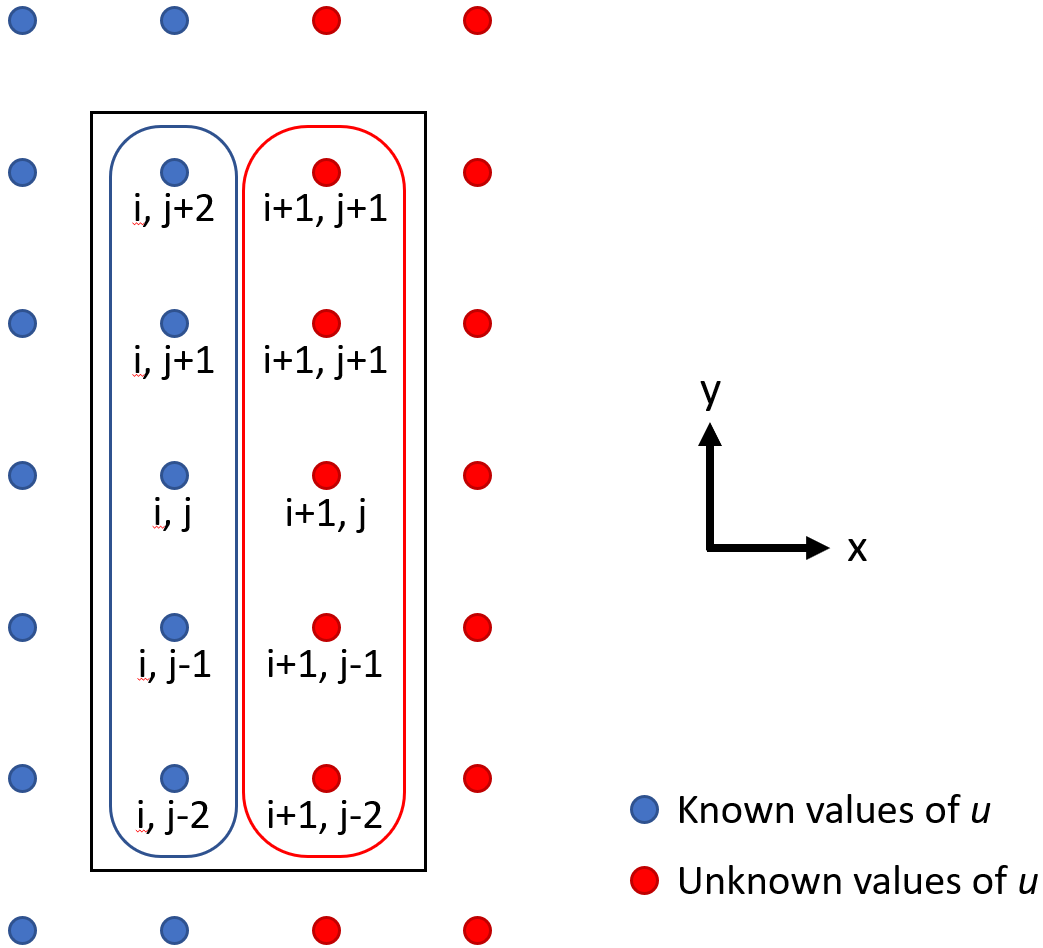
\includegraphics[width=6cm]{stencil.PNG}
  		\caption{The computational stencil for internal nodes. The Crank-Nicolson scheme uses information at the \textit{$i^{th}$} column to calculate all values at \textit{i+1}.}
  		\label{stencil}
	\end{center}
\end{figure}

\vspace{11pt}
These equations are assembled into a matrix equation \textit{$\underline{\underline{A}}^{ } \underline{u_{i+1}} = \underline{b}$} and the matrix equation is solved by inverting the coefficient matrix \textit{A} and multiplying the result by \textit{b}. 

\vspace{-5pt}
\begin{equation}
\underline{u_{i+1}} = \underline{\underline{A}}^{-1} \underline{b}
\end{equation}

For the first internal node near a boundary, in which there are fewer than two nodes above or below, a second-order central differencing scheme was used. The computational stencil for a boundary node is shown in Figure \ref{stencil_boundary}. 

\begin{figure}[H]
	\begin{center}
		\includegraphics[width=6cm]{stencil_boundary.PNG}
  		\caption{The computational stencil for nodes near boundaries.}
  		\label{stencil_boundary}
	\end{center}
\end{figure}

A code was written in Python to systematically loop through all nodes in the y-direction and to assemble the coefficient matrix. The full Python code is available in Appendix 1. For each x-step, the coefficient matrix must be inverted to solve for the values of \textit{u} at the \textit{i+1} step.
\bigskip

The form of the \textit{A} matrix is pentadiagonal, because there are five unknowns for each location of the stencil. While standard matrix inversion algorithms exist, a code designed specifically to solve a pentadiagonal matrix would theoretically reduce the number of computations and save calculation time.

\subsection*{LU Decomposition Matrix Inversion Algorithm}
\vspace{-5pt}
To invert the matrix, an LU decomposition scheme was written specifically for a pentadiagonal matrix. The widely-known LU decomposition algorithm was modified to reduce the number of floating-point operations, because the input matrix is known to be pentadiagonal. The full derivation of LU decomposition will not be shown, but the process will be summarized here. In this method, the matrix \textit{A} is set equal to the matrix product of \textit{L}, a lower triangular matrix, and \textit{U}, an upper triangular matrix. Because triangular matrices are much easier to invert than a dense matrix, the LU decomposition is a direct method that allows the exact matrix inverse to be calculated. In general, the process is as follows:

\begin{equation}
\underline{\underline{L}}^{ } \underline{\underline{U}} \underline{u_{i+1}} = \underline{b} \Rightarrow \underline{\underline{U}}^{ } \underline{u_{i+1}} = \underline{\underline{L}}^{-1}\underline{b} \Rightarrow \underline{u_{i+1}} = \underline{\underline{U}}^{-1}(\underline{\underline{L}}^{-1}\underline{b})
\end{equation}

This process is used to solve for the \textit{$u_{i+1}$} values in each x-step. The LU decomposition algorithm was implemented in the Python code.

%%%%%%%%%%%%%%%%%%%%%%%%%%%%%%%%%%%%%%%%%%%%%%%%%%%%%%%%%%%%%%%%%%%%%%
\vspace{-5pt}
\section*{Results}
\vspace{-8pt}
Initially, a coarse grid with 21 nodes in the x-direction and 21 nodes in the y-direction was used to calculate results. A contour plot of \textit{u} as a function of x and y is shown in Figure \ref{contour21}, and a 1-dimensional plot of \textit{u(y)} at \textit{x} = 0.05, 0.1, 0.2, 0.5, and 1.0 is shown in Figure \ref{curves21}. The boundary conditions are satisfied by this result. At low values of x, u(y) is changing the most dramatically. As x increases, the profile of u(y) settles to a slightly upward-curving shape. At x = 0.5, the curve changes minimally though the remainder of the computational domain; the curves for x = 0.5 and x = 1.0 are indistinguishable. The absolute error in the numerical solution, defined as the absolute value of the numerical solution minus the analytical solution, is shown in Figures \ref{err_contour21} and \ref{err_curves21}.

\begin{figure}[H]
\centering
\begin{minipage}{.49\textwidth}
  \centering
  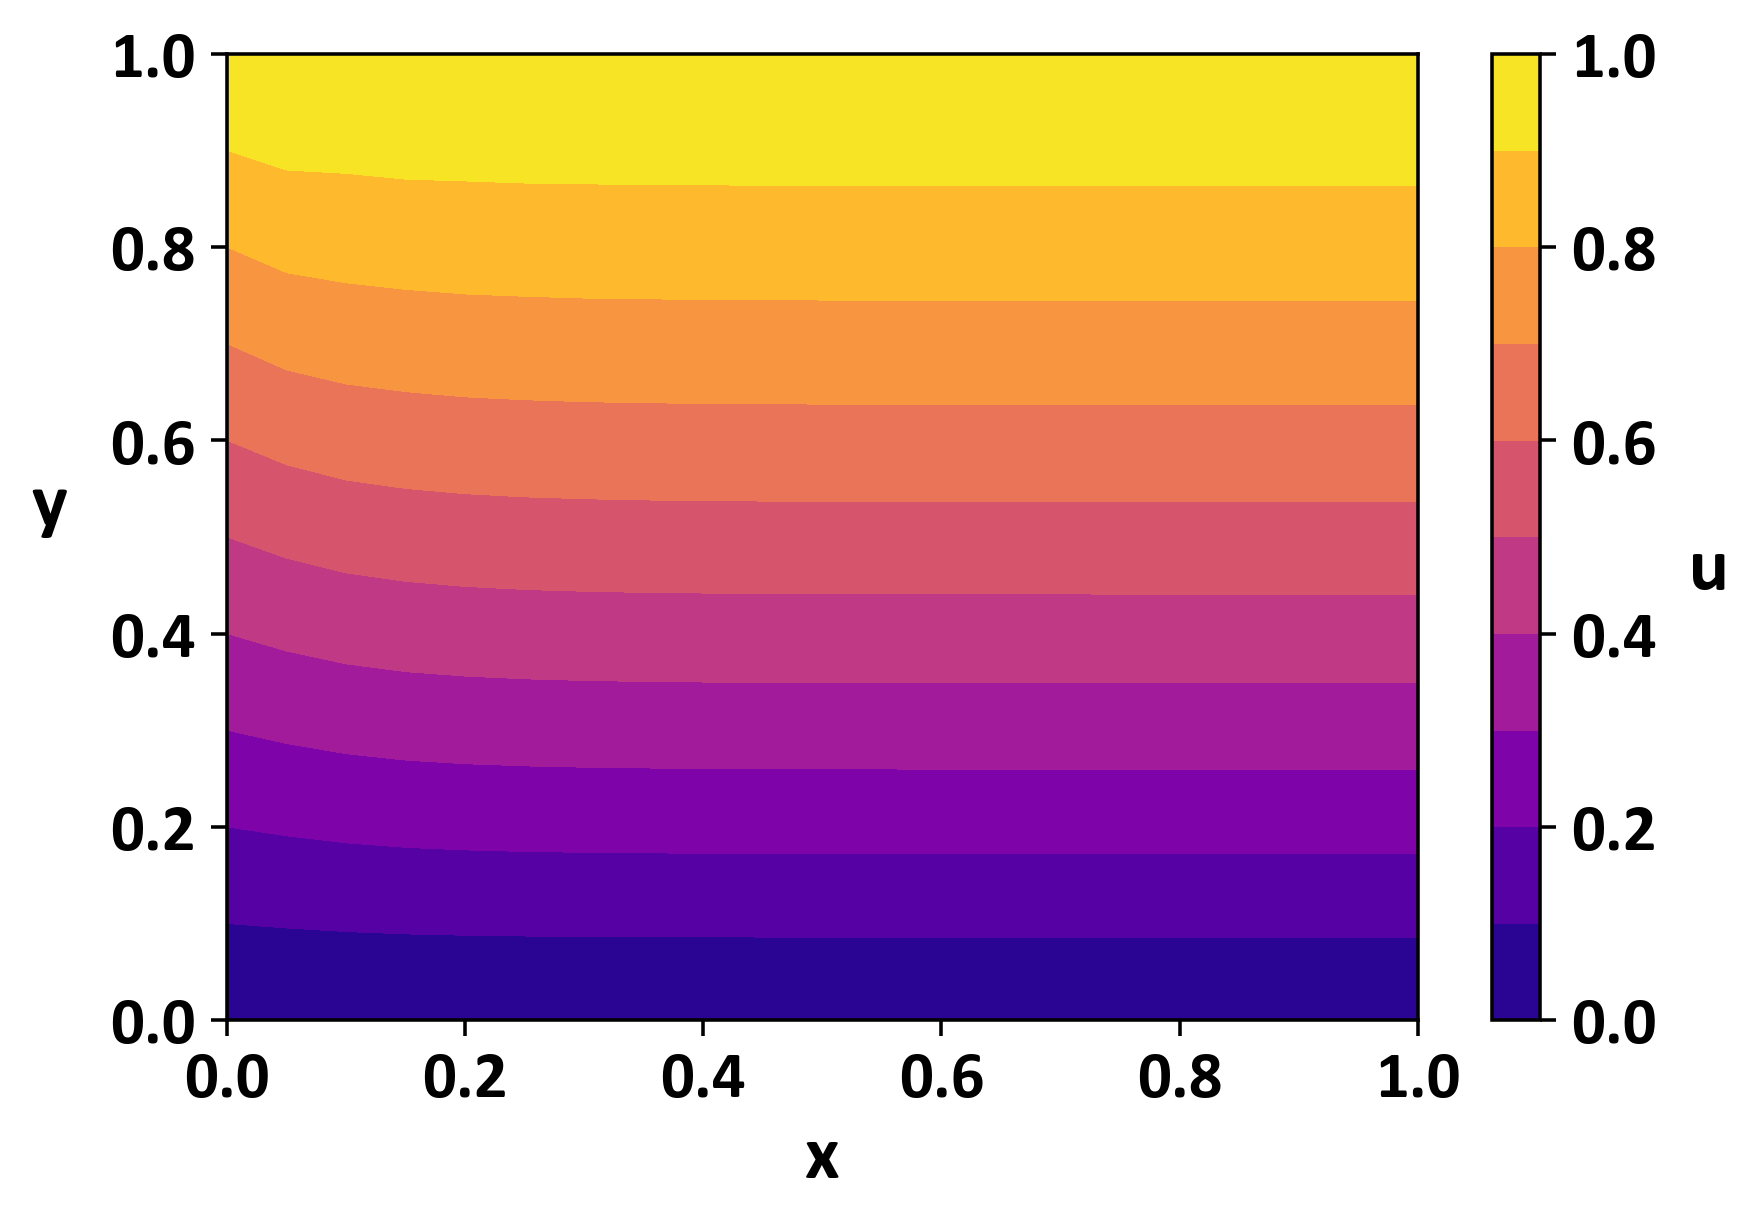
\includegraphics[width=.9\linewidth]{contour21_21.png}
  \captionsetup{width=.95\linewidth}
  \captionof{figure}{Numerical solution of \textit{u} with $N_x$ = 21 and $N_y$ = 21.}
  \label{contour21}
\end{minipage}
\begin{minipage}{.49\textwidth}
  \centering
  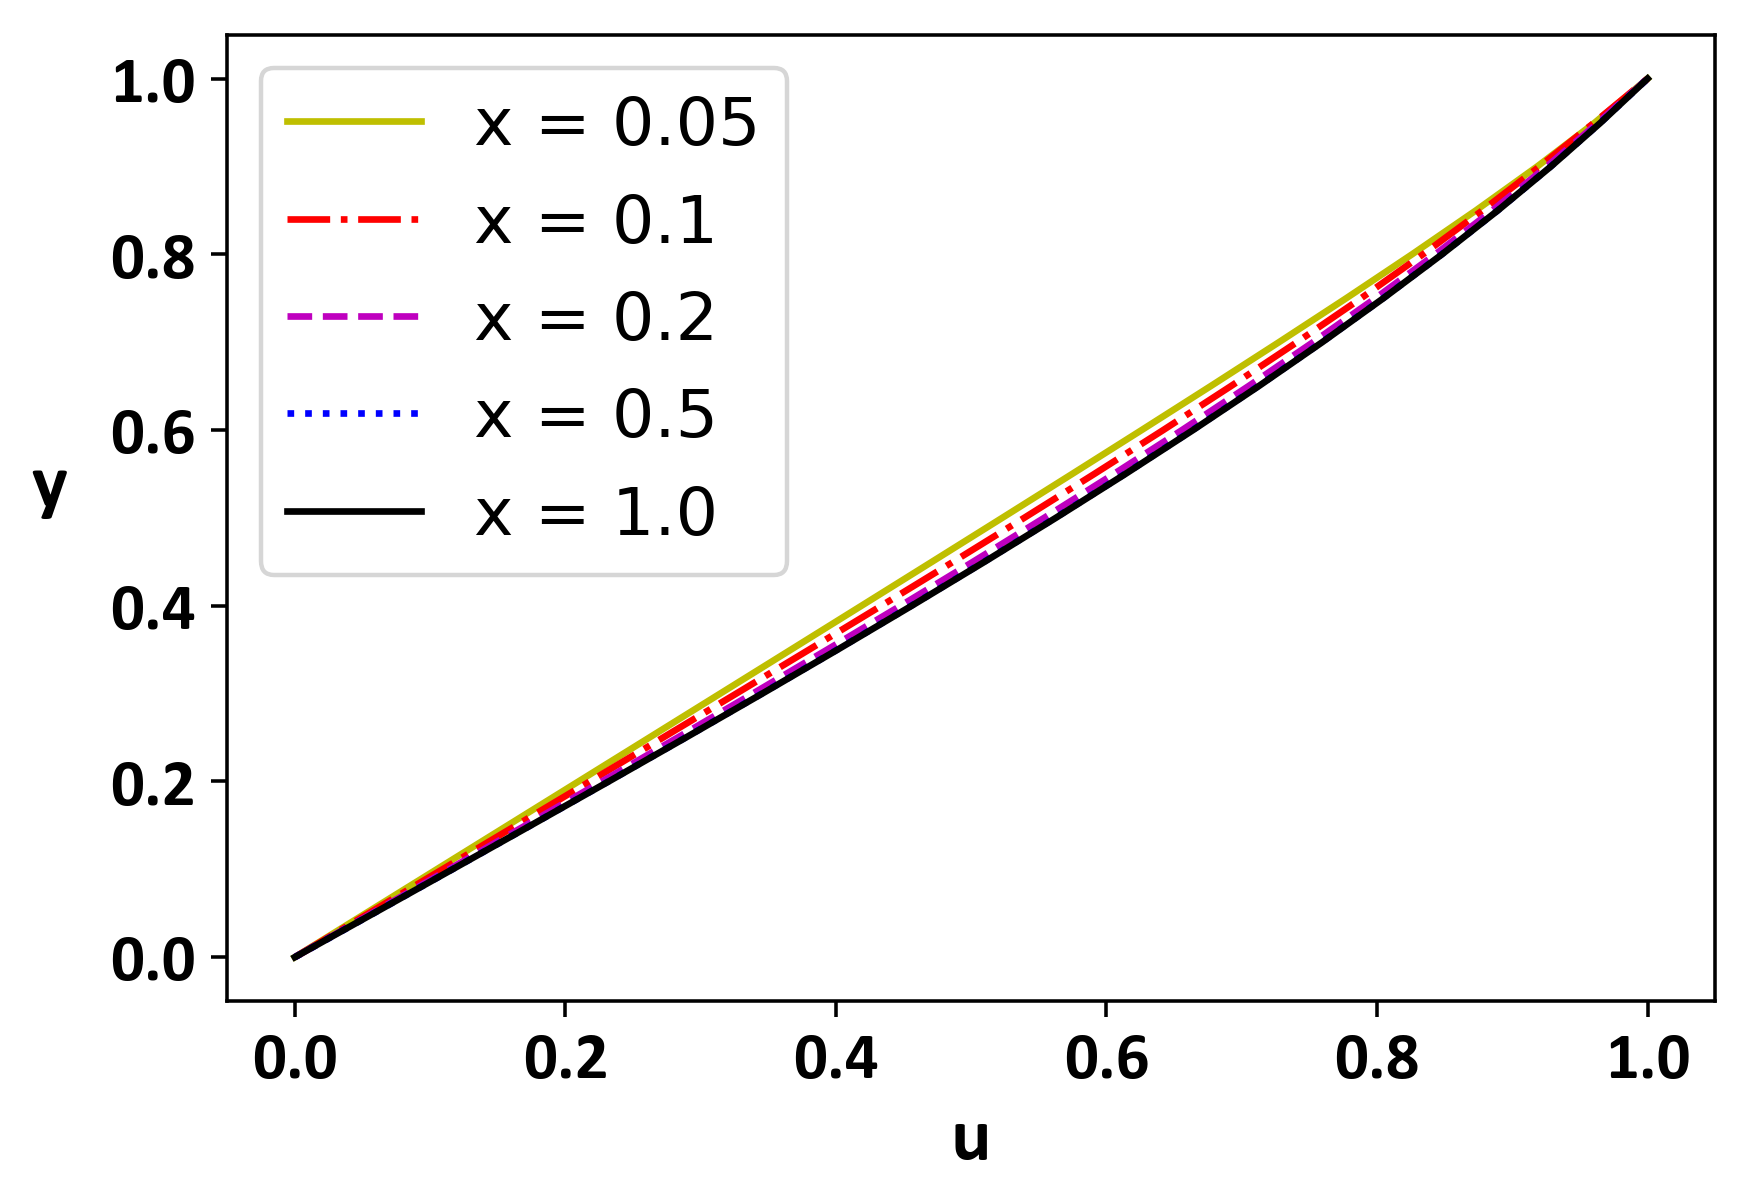
\includegraphics[width=.9\linewidth]{curves21_21.png}
  \captionsetup{width=.95\linewidth}
  \captionof{figure}{Numerical solution of \textit{u} with $N_x$ = 21 and $N_y$ = 21 at x = 0.05, 0.1, 0.2, 0.5, and 1.0.}
  \label{curves21}
\end{minipage}
\end{figure}

\begin{figure}[H]
\centering
\begin{minipage}{.49\textwidth}
  \centering
  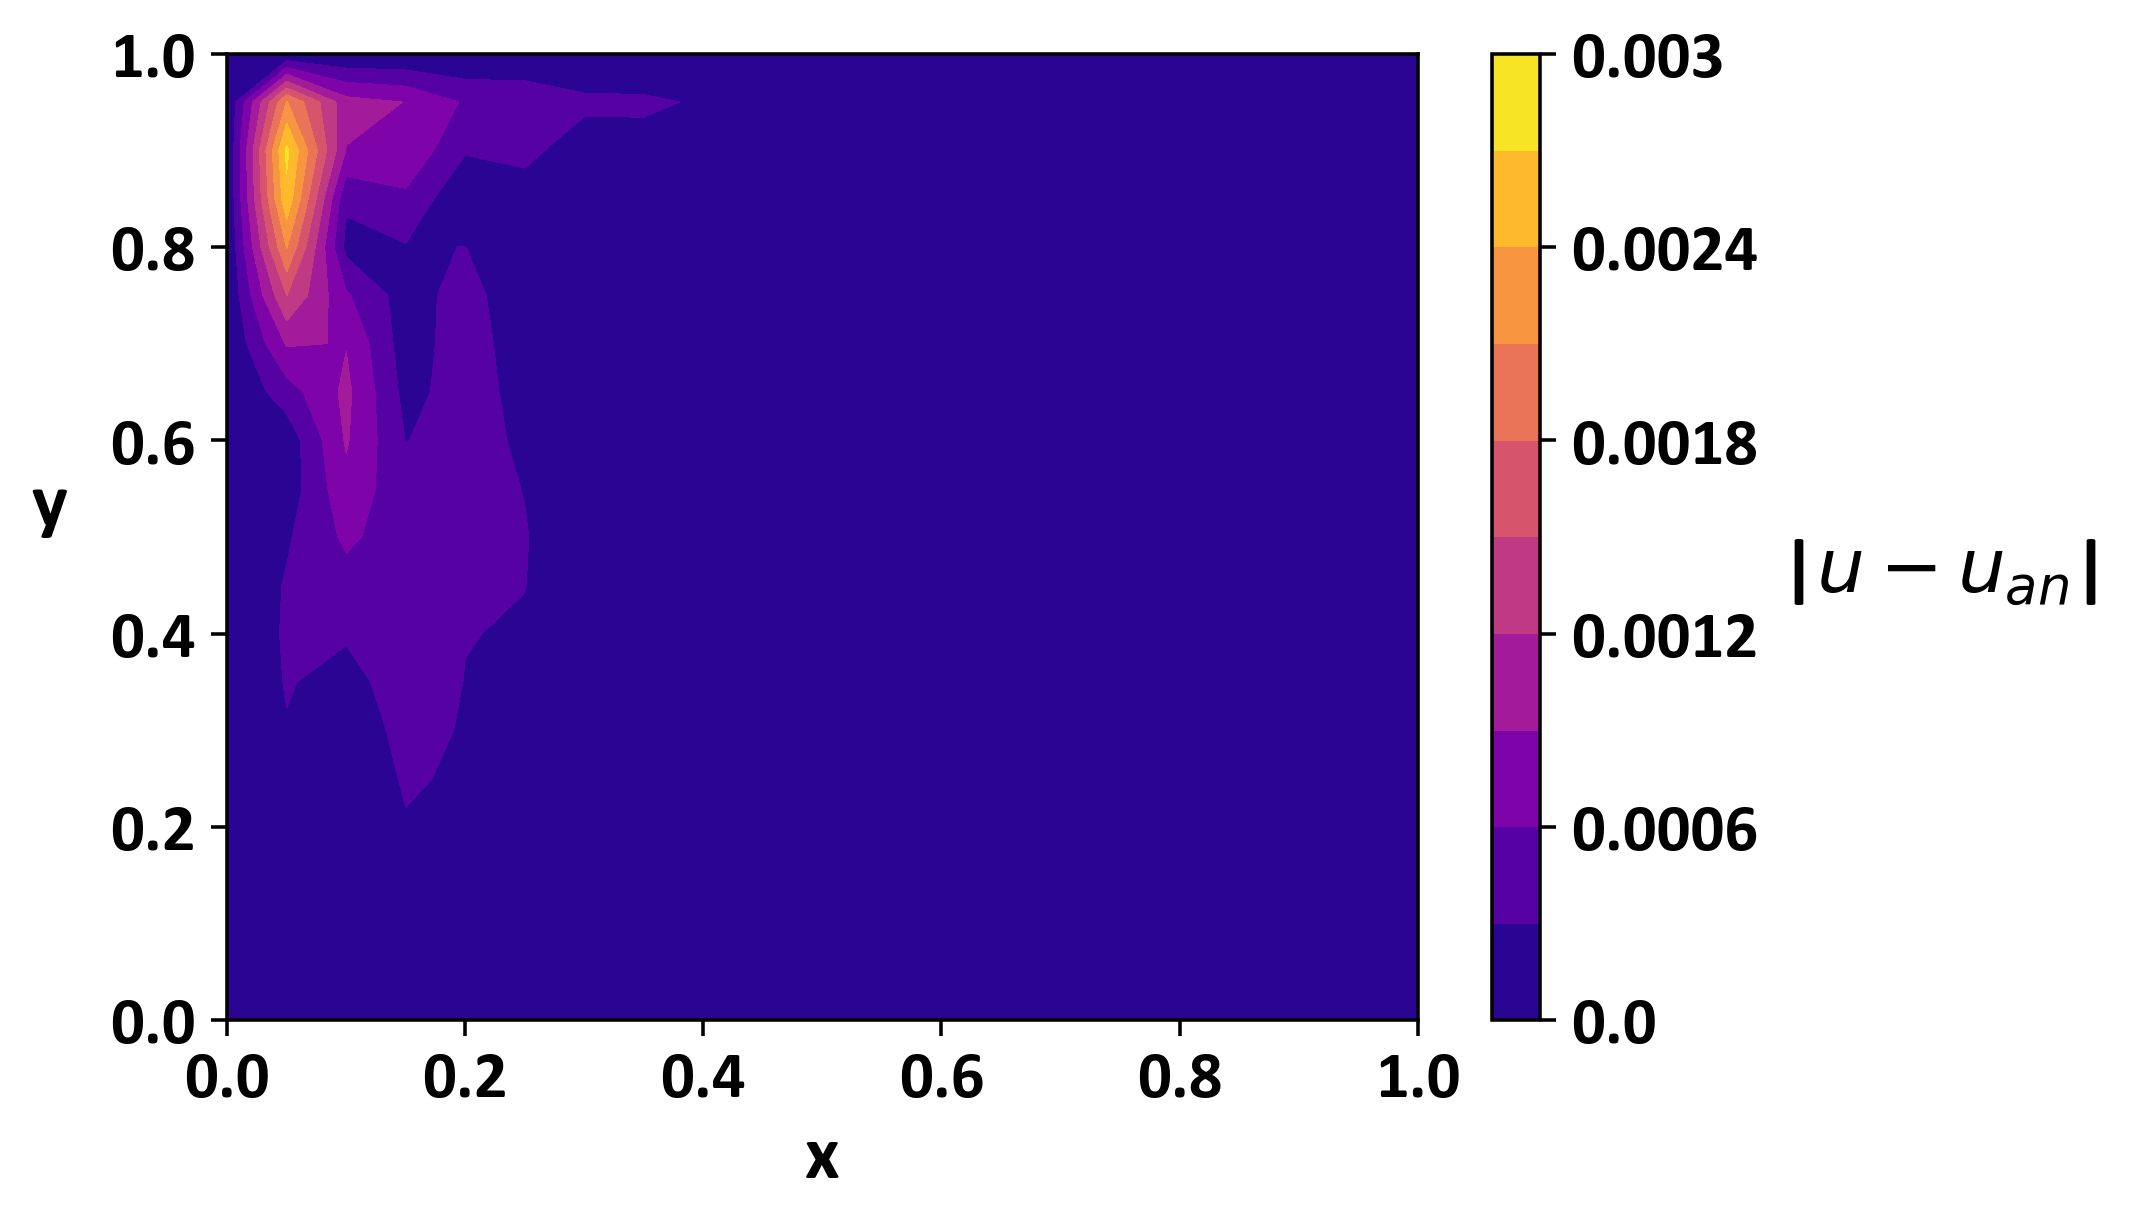
\includegraphics[width=1\linewidth]{err_contour21_21.png}
  \captionsetup{width=.95\linewidth}
  \captionof{figure}{Error in numerical solution of \textit{u} with \break $N_x$ = 21 and $N_y$ = 21.}
  \label{err_contour21}
\end{minipage}
\begin{minipage}{.49\textwidth}
  \centering
  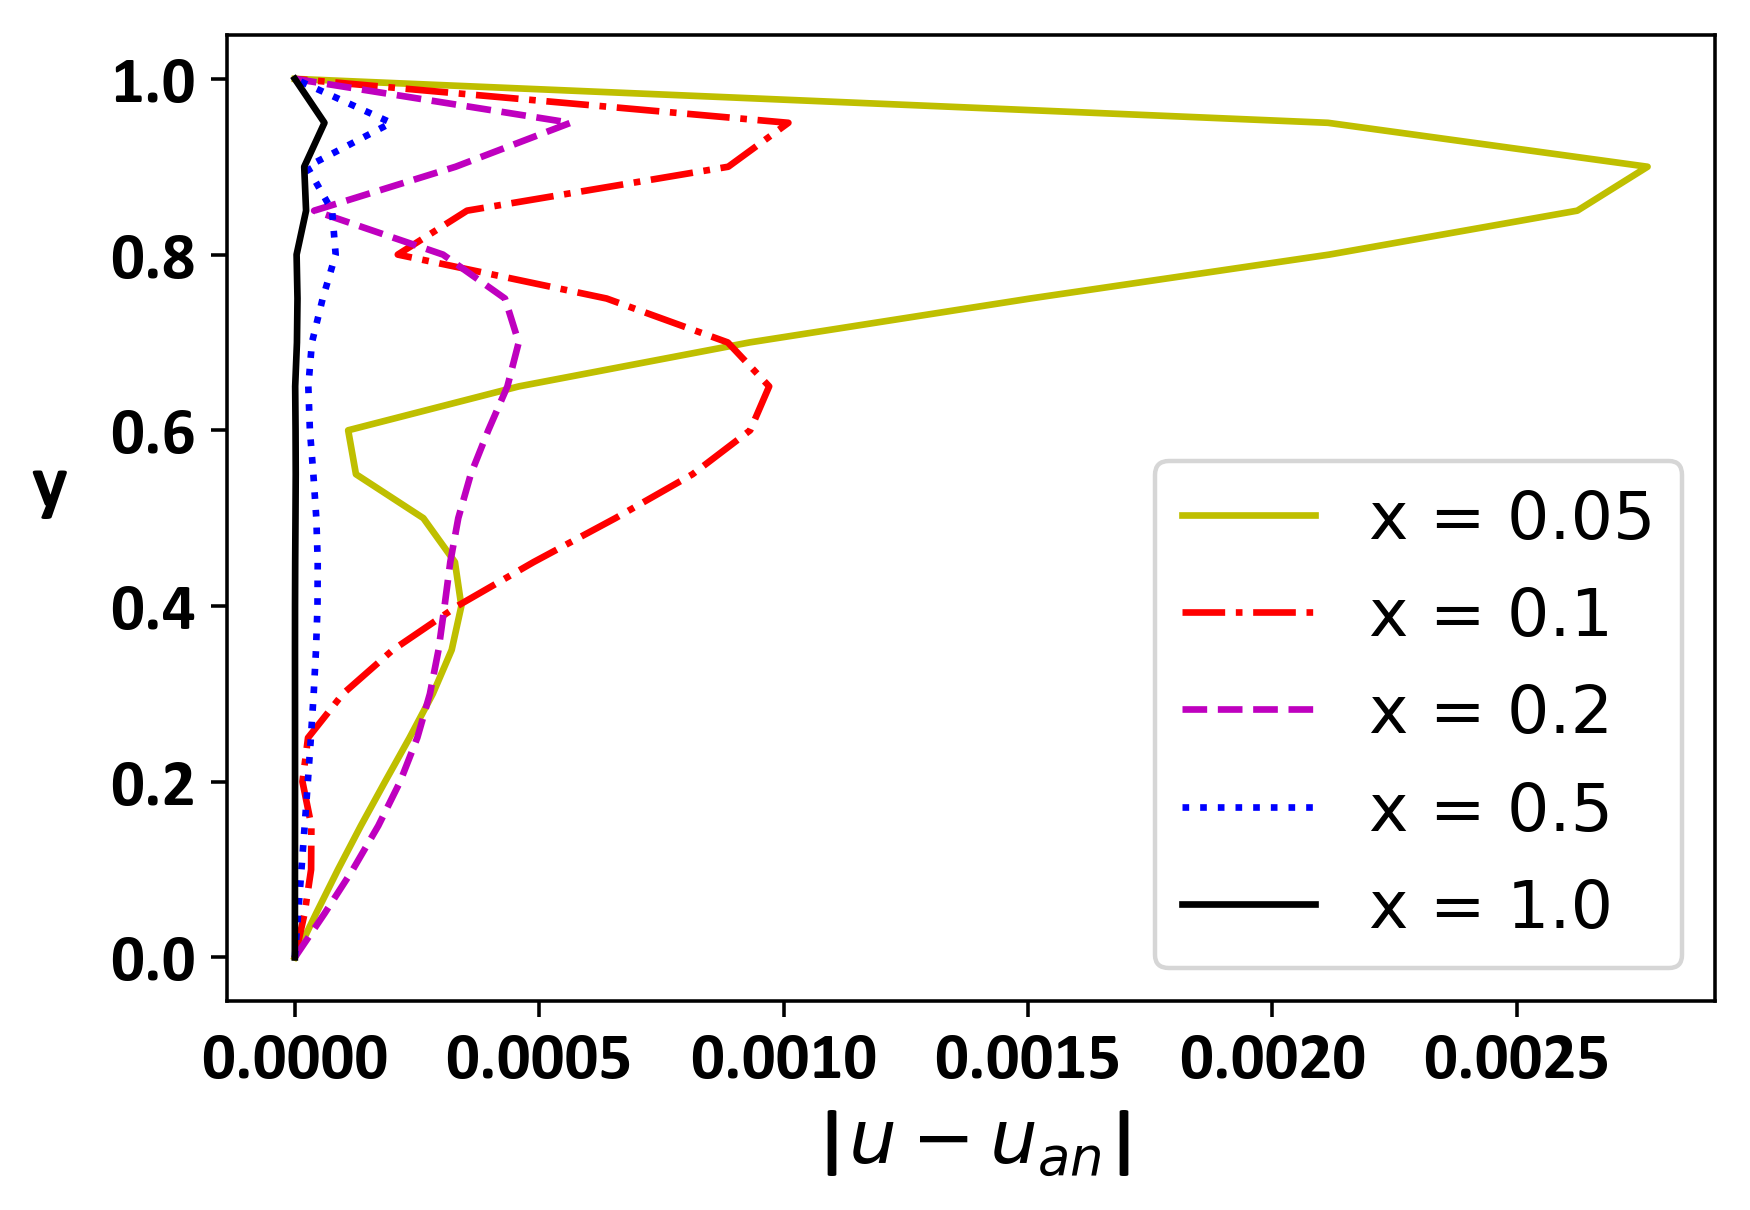
\includegraphics[width=.8\linewidth]{err_curves21_21.png}
  \captionsetup{width=.95\linewidth}
  \captionof{figure}{Error in numerical solution of \textit{u} with \break $N_x$ = 21 and $N_y$ = 21 at x = 0.05, 0.1, 0.2, 0.5, and 1.0.}
  \label{err_curves21}
\end{minipage}
\end{figure}

The maximum relative error is approximately 0.3\%, so even with a coarse grid the results are quite accurate. The regions with the the steepest gradients (near x = 0.05 and y = 0.9) have the highest error, as expected. As the solution increases in x, the error decreases and the numerical solution is in very good agreement with the analytical solution.

\subsection*{Effect of Grid Spacings $\Delta x$ and $\Delta y$}
\vspace{-5pt}

The effect of grid spacings $\Delta x$ and $\Delta y$ were studied by first varying $\Delta x$ while $\Delta y$ was held constant, then varying $\Delta y$ while $\Delta x$ was held constant, and finally decreasing both $\Delta x$ and $\Delta y$ together as the same values. Figure \ref{dxEffect} shows that decreasing $\Delta x$ decreases error up until a certain limit. Eventually the accuracy of the solution is limited by the finite-precision numbers used by the computer, and the error no longer increases. Also as $\Delta x$ decreases, the computation time increases exponentially. Figure \ref{dyEffect} shows that decreasing $\Delta y$ does not decrease error. This would lead one to conclude that $\Delta x$ is the key factor that determines error. Similarly to Figure \ref{dxEffect}, the computation time increases exponentially as $\Delta y$ decreases. Figure \ref{dxdyEffect} shows the effect on error and computation time as both $\Delta x$ and $\Delta y$ are decreased together. The error is comparable to Figure \ref{dxEffect}, in which only $\Delta x$ was changed, while the computational effort is orders of magnitude higher. The lack of improvement in error with dramatically increased computation time indicates that the lowest error should be pursued by decreasing $\Delta x$ only.

\begin{figure}[H]
\centering
\begin{minipage}{.49\textwidth}
  \centering
  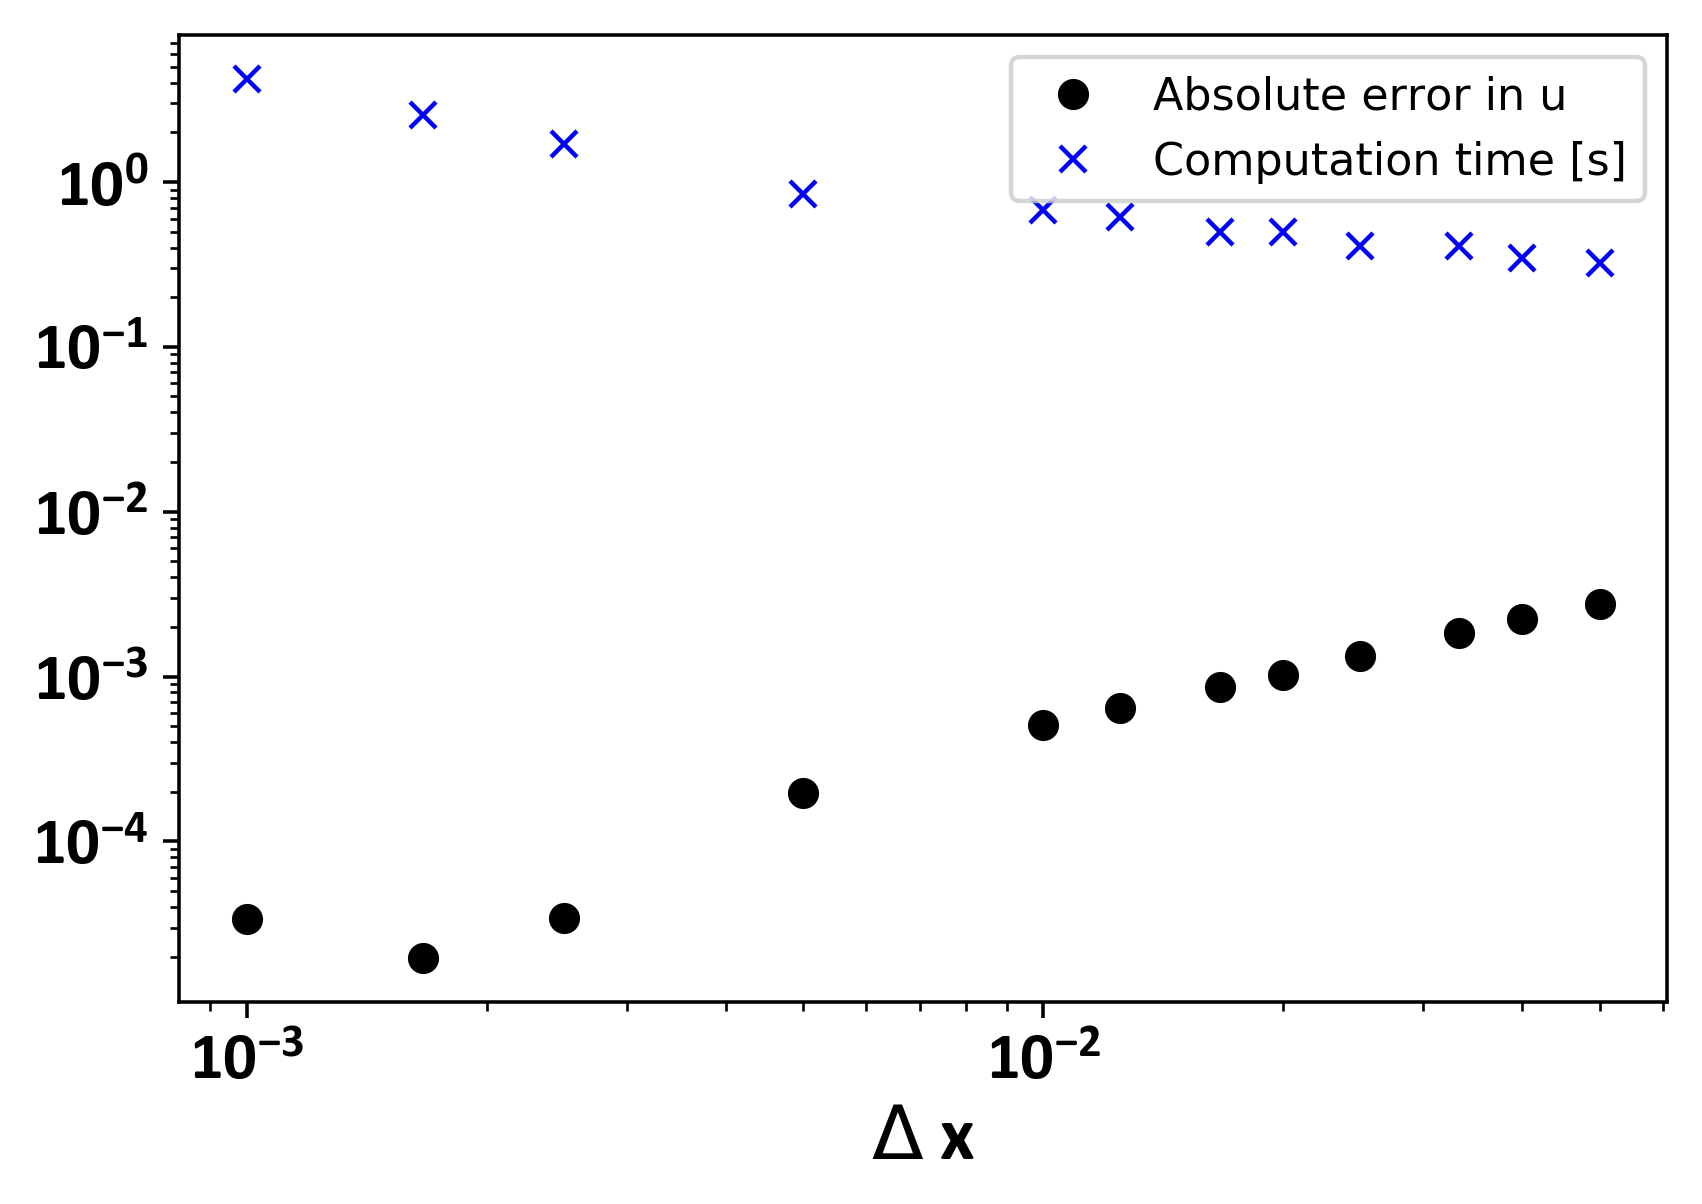
\includegraphics[width=.87\linewidth]{dxEffect.png}
  \captionsetup{width=.95\linewidth}
  \captionof{figure}{Effect of varying $\Delta$x on error and computation time with $\Delta$y held constant at 0.05.}
  \label{dxEffect}
\end{minipage}
\begin{minipage}{.49\textwidth}
  \centering
  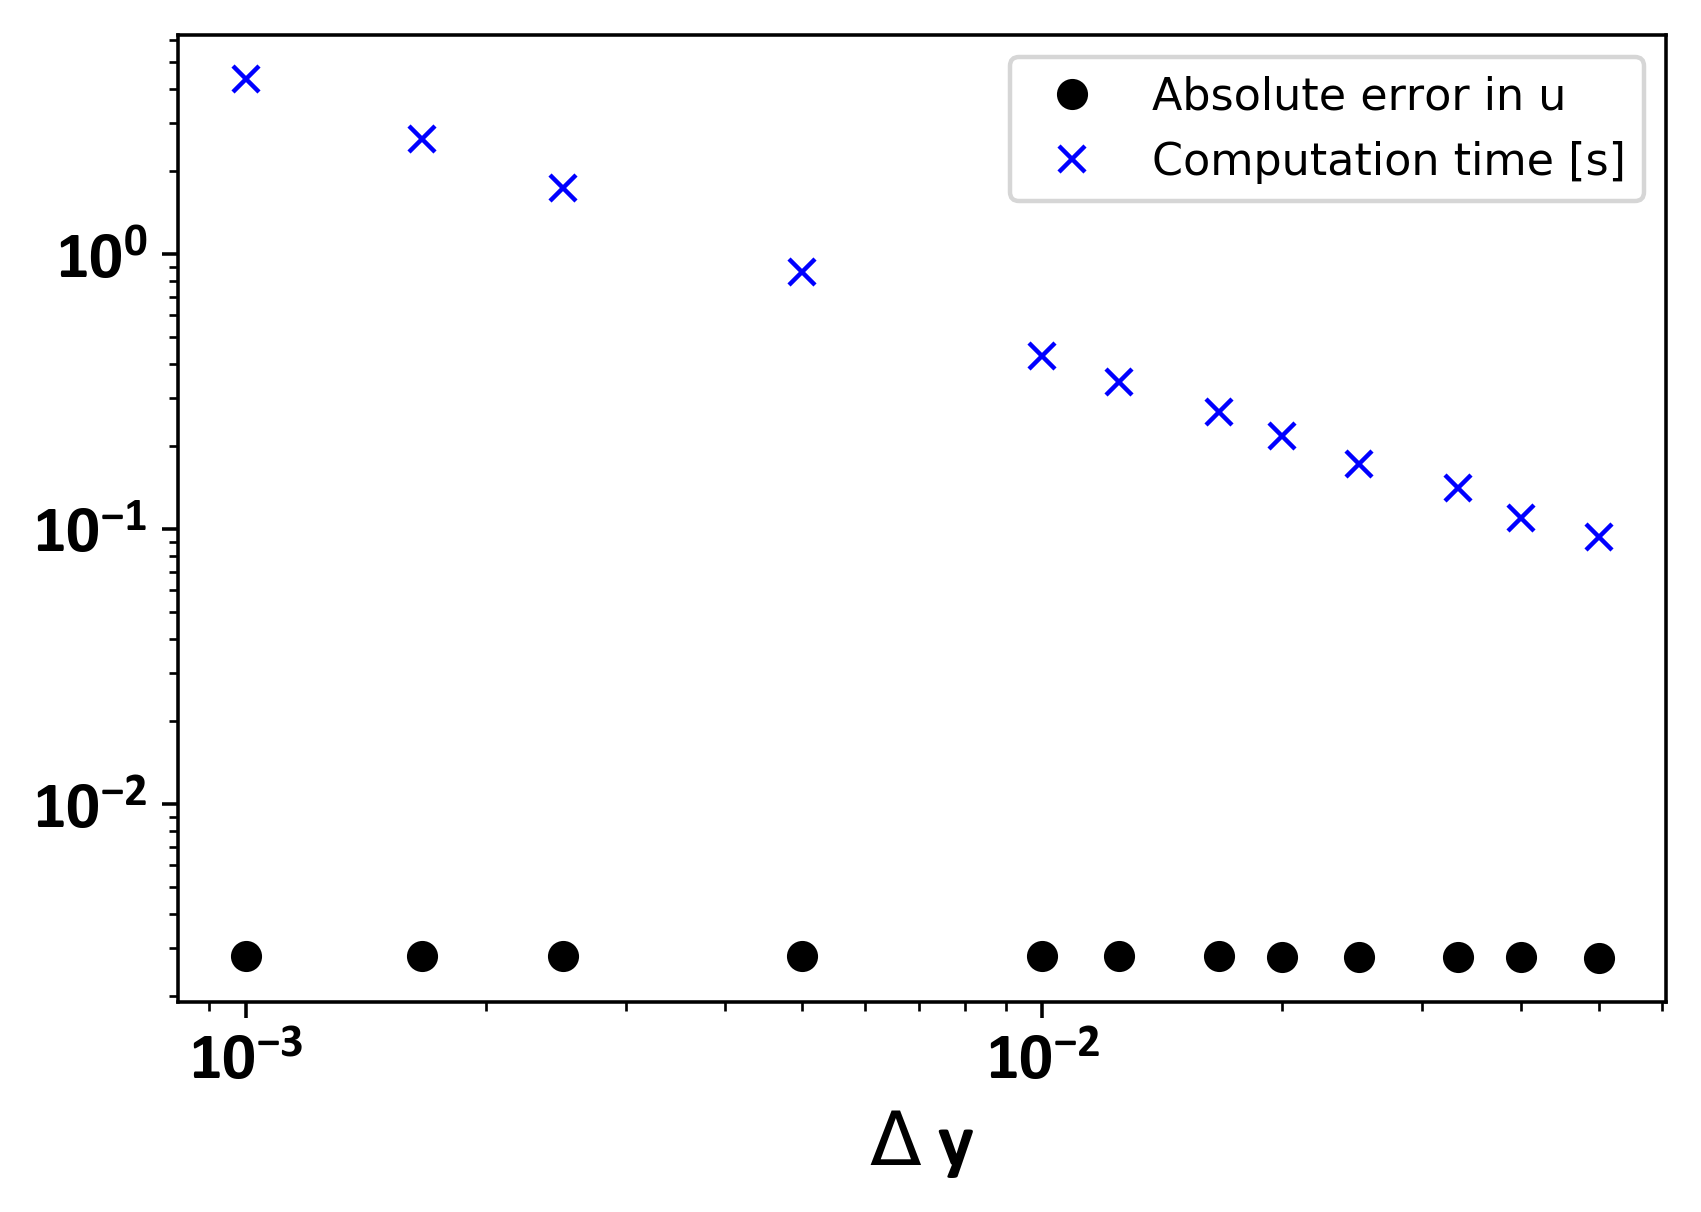
\includegraphics[width=.87\linewidth]{dyEffect.png}
  \captionsetup{width=.95\linewidth}
  \captionof{figure}{Effect of varying $\Delta$y on error and computation time with $\Delta$x held constant at 0.05.}
  \label{dyEffect}
\end{minipage}
\end{figure}

\begin{figure}[H]
	\begin{center}
		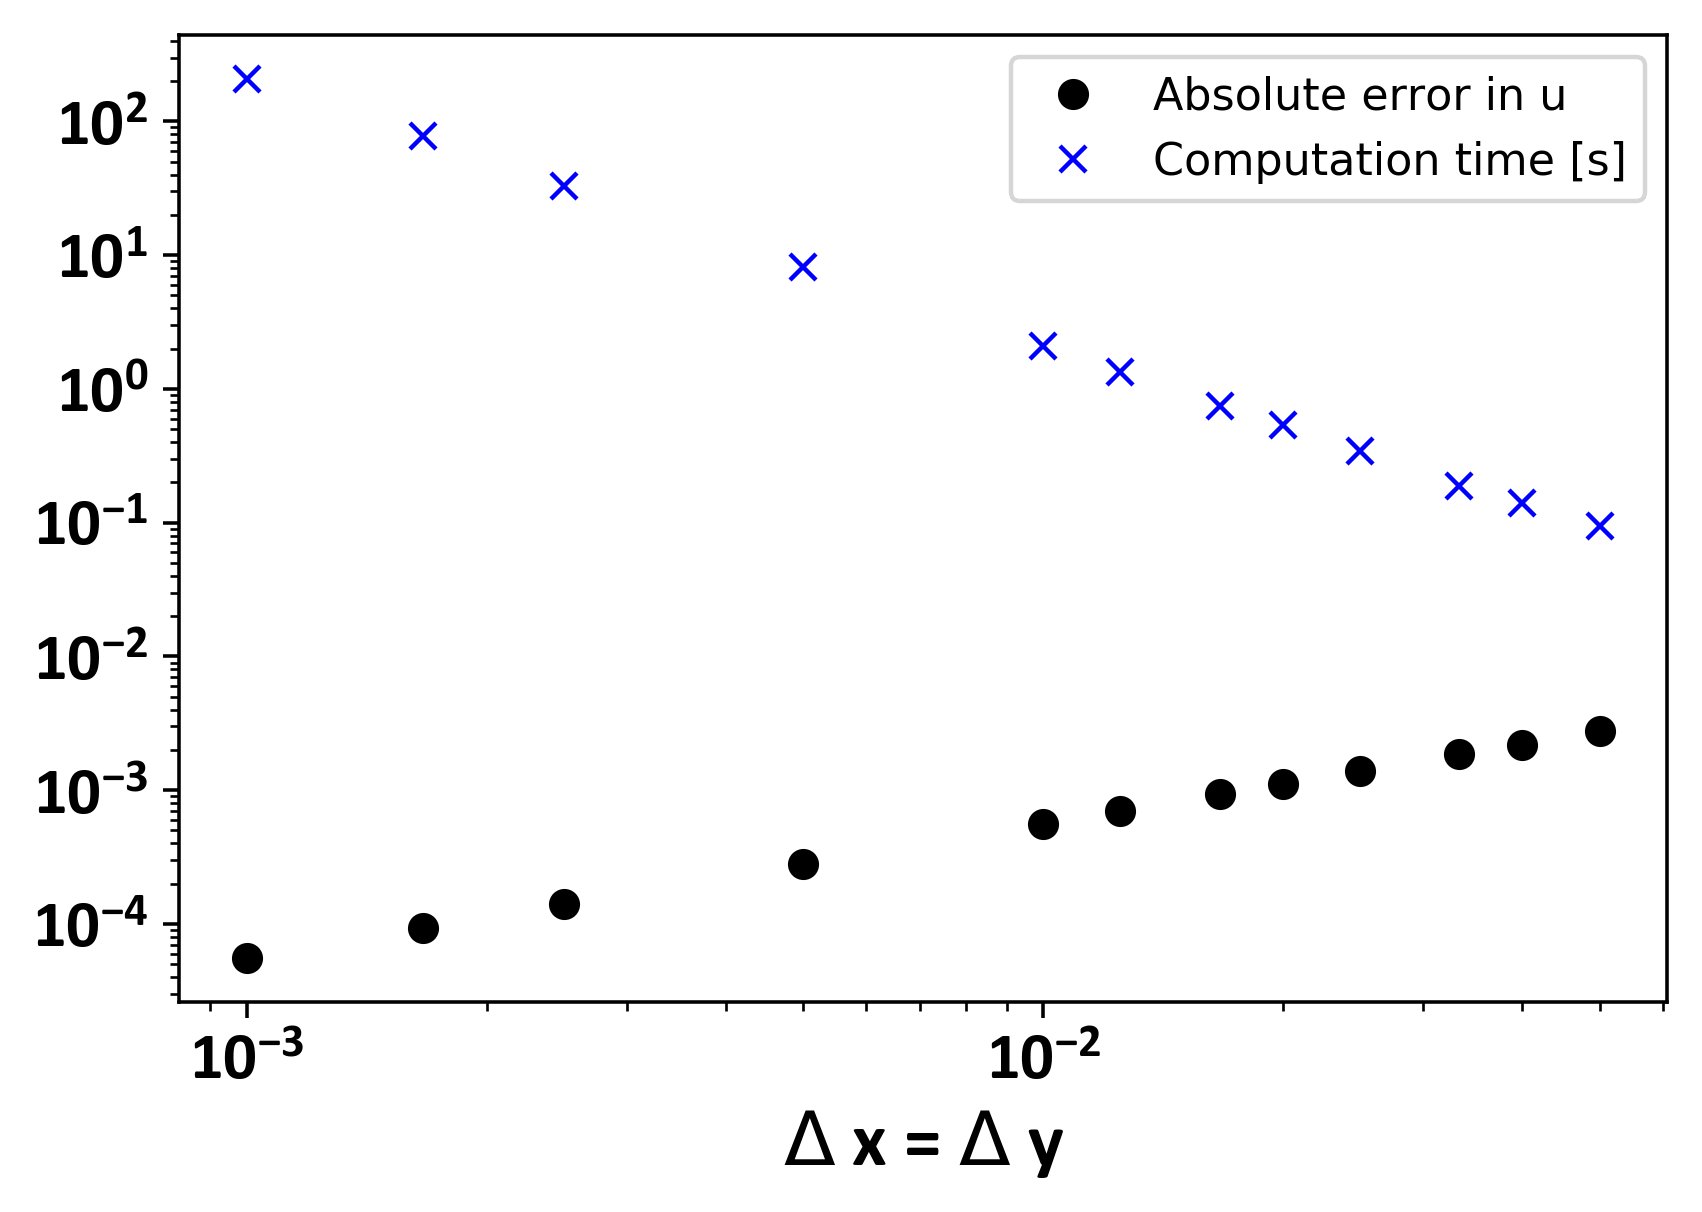
\includegraphics[width=7cm]{dxdyEffect.png}
  		\caption{Effect of varying $\Delta$x and $\Delta$y together on error and computation time}
  		\label{dxdyEffect}
	\end{center}
\end{figure}

%%%%%%%%%%%%%%%%%%%%%%%%%%%%%%%%%%%%%%%%%%%%%%%%%%%%%%%%%%%%%%%%%%%%%%
\section*{Conclusion}
\vspace{-8pt}
A finite-difference code was written in Python to solve a linear, non-homogeneous parabolic partial differential equation. First, the analytical solution was solved using superposition, separation of variables, and orthogonality to result in an infinite Fourier sine series solution. The numerical method used a fourth-order central difference approach in y with a Crank-Nicolson algorithm to march in x, utilizing LU decomposition to solve for a column of \textit{u}-values simultaneously at each x-step. A coarse grid was found to resolve the solution to a high degree of accuracy. The areas of the solution with the steepest gradients had the largest errors in the numerical solution. Decreasing x-spacing $\Delta x$ had a direct effect on reducing error in the solution, while decreasing $\Delta y$ had no effect on error. Decreasing either spacing resulted in significant increases to computation time.


\pagebreak
\section*{Appendix 1: Python Code}

\inputminted{python}{project1.py}

\pagebreak
\section*{Appendix 2: Derivation of Analytical Solution}
\begin{figure}[H]
	\begin{center}
		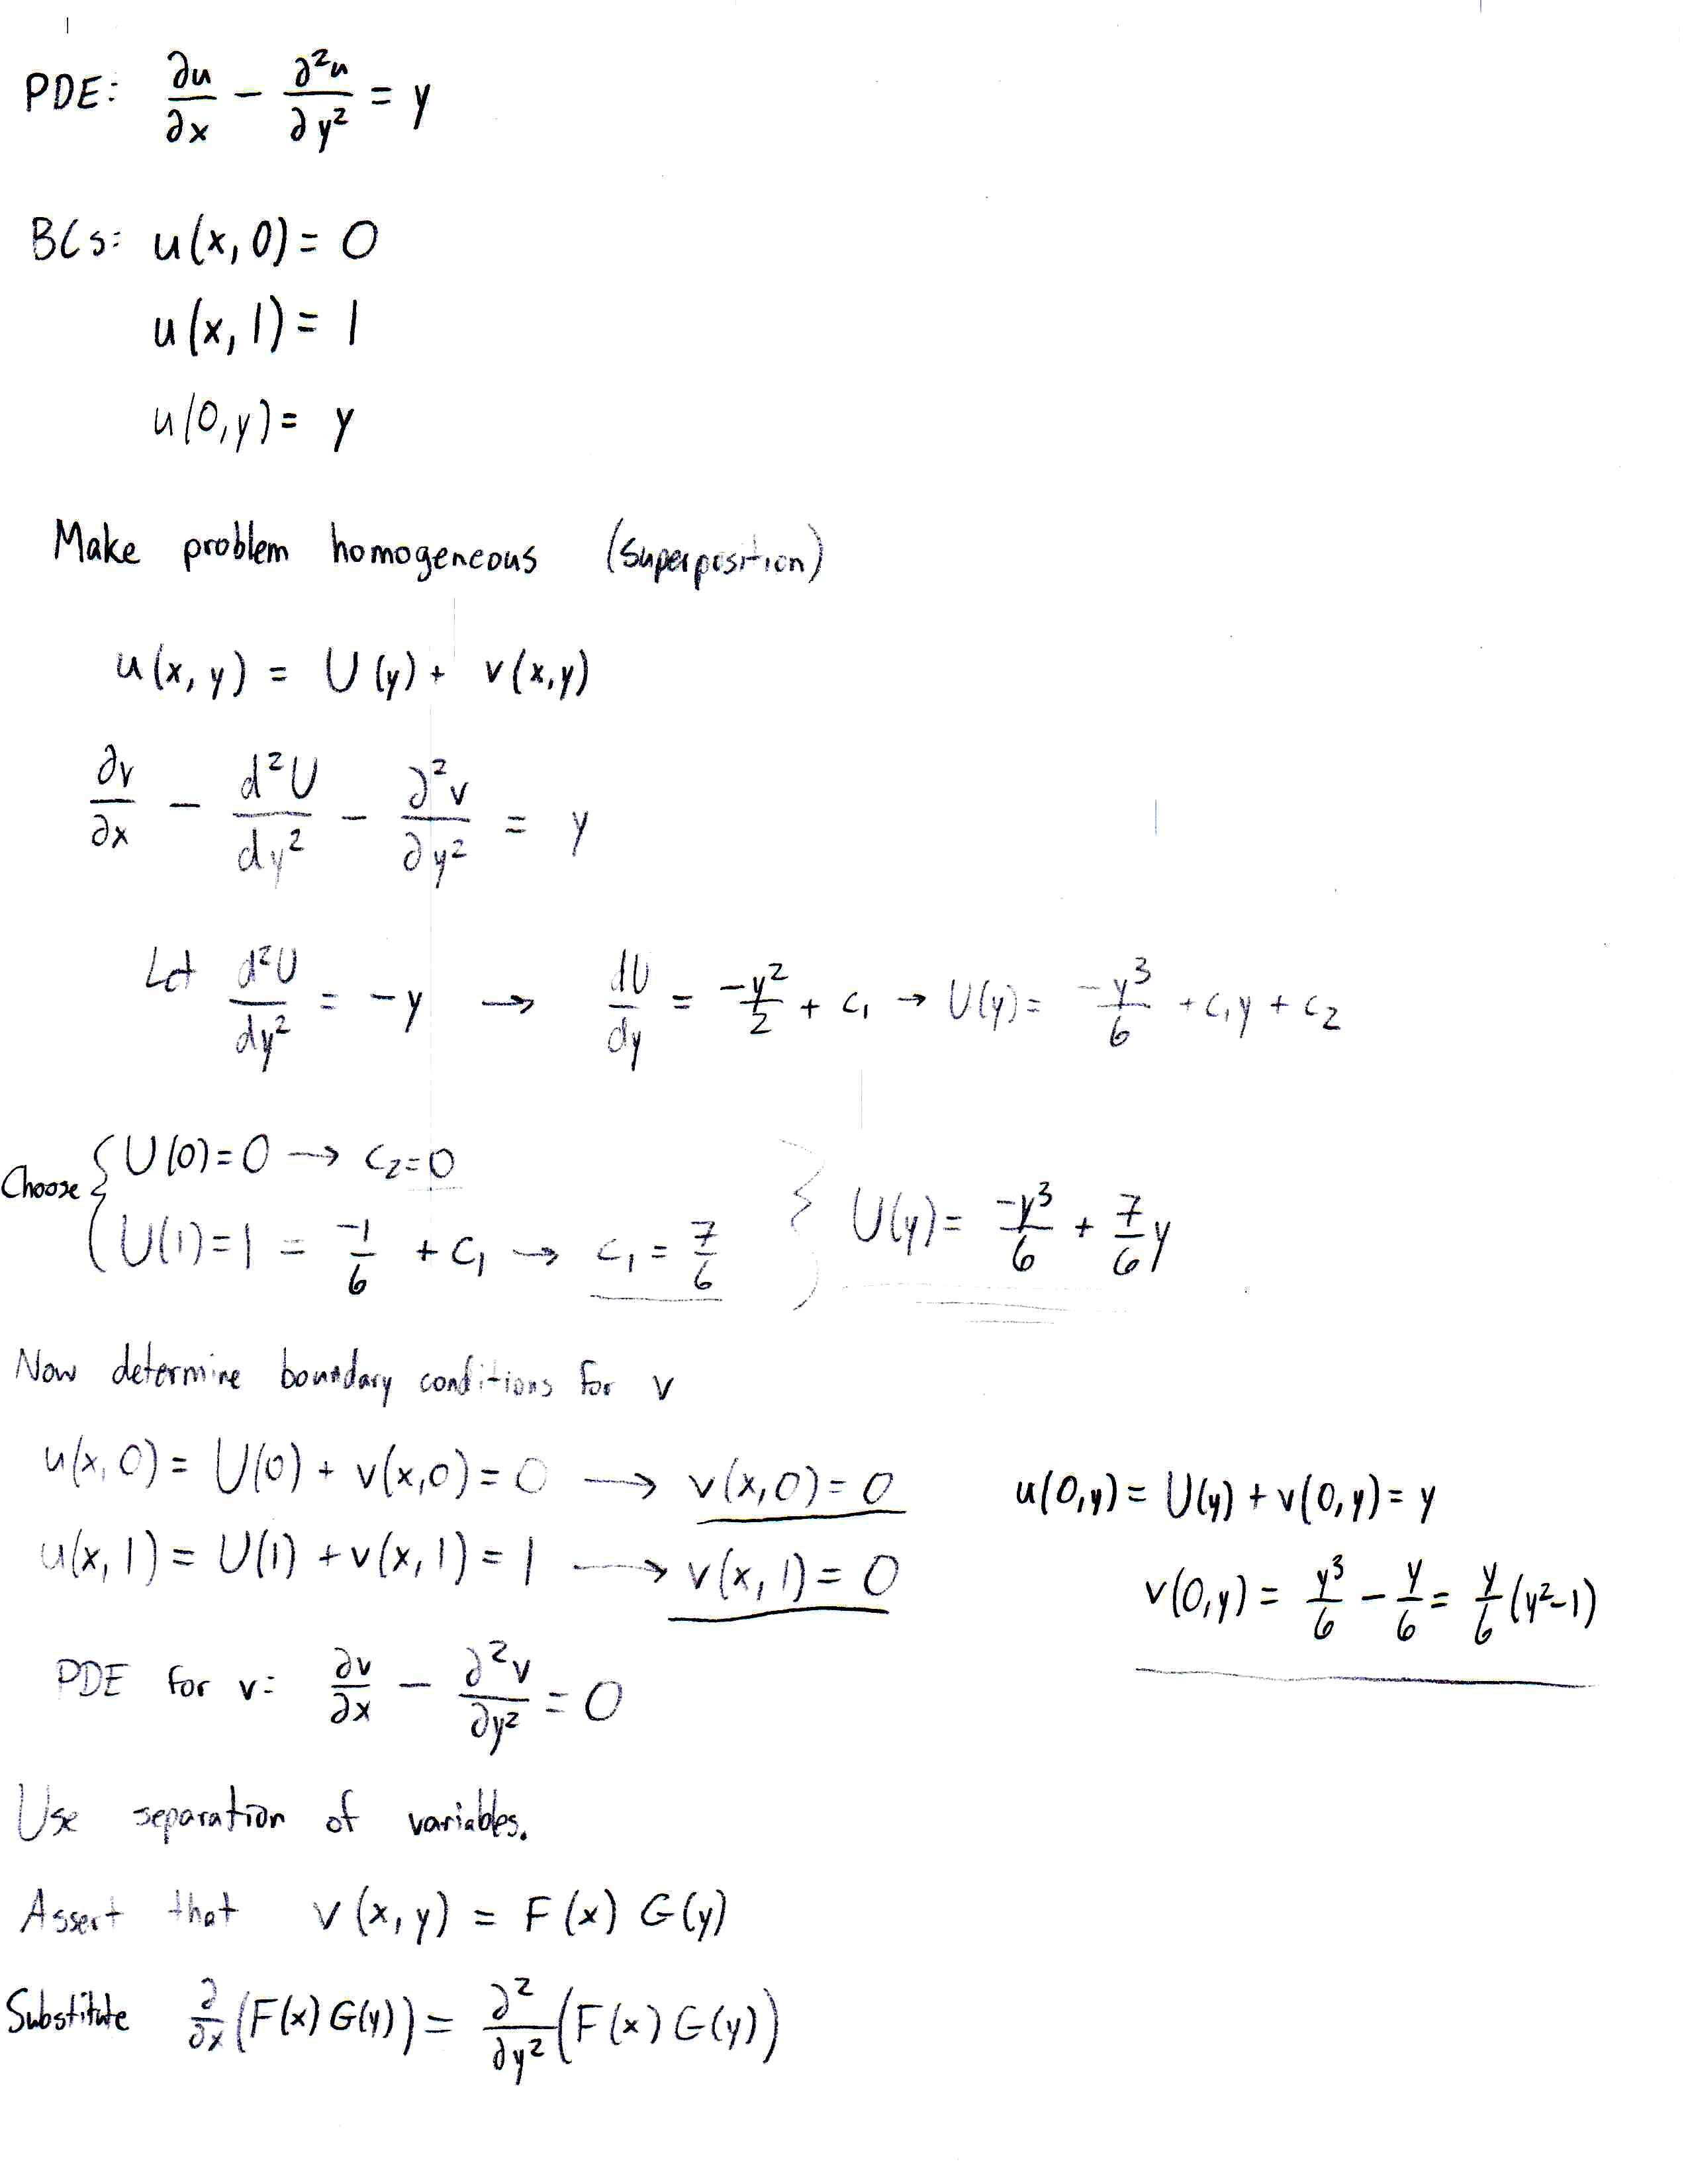
\includegraphics[width=16cm]{app2_p1.jpg}
	\end{center}
\end{figure}
\pagebreak
\begin{figure}[H]
	\begin{center}
		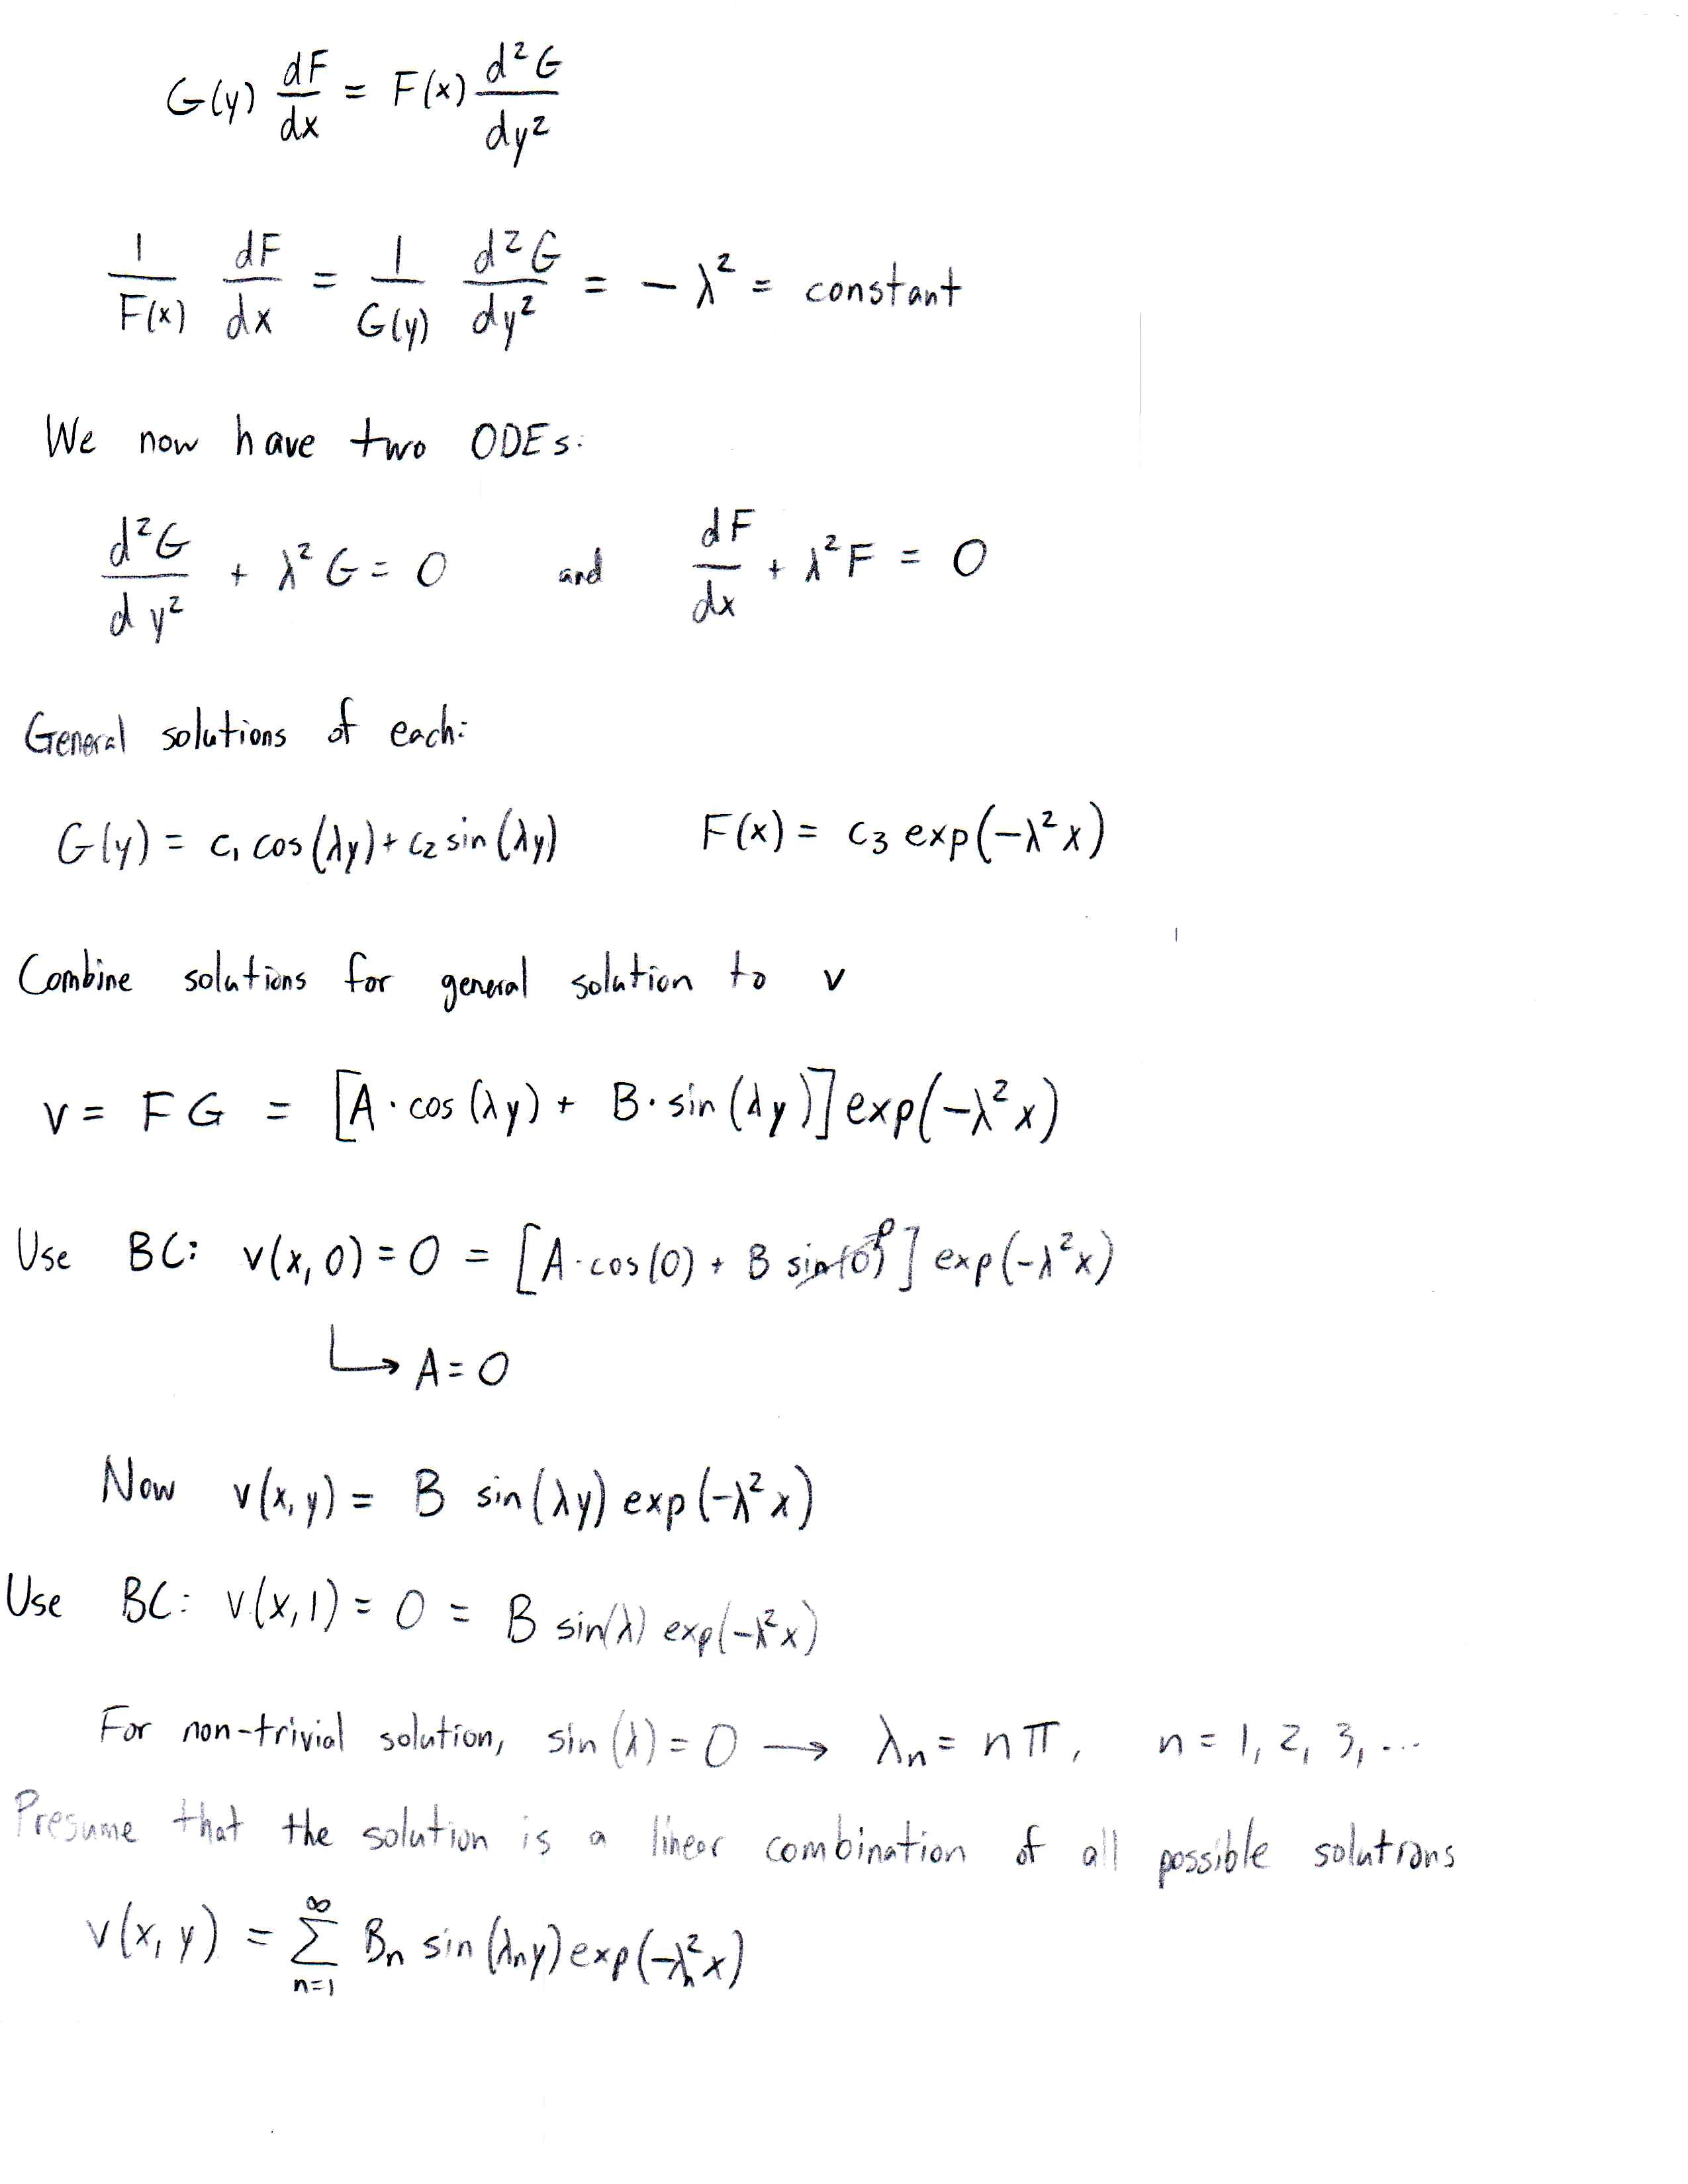
\includegraphics[width=16cm]{app2_p2.jpg}
	\end{center}
\end{figure}
\pagebreak
\begin{figure}[H]
	\begin{center}
		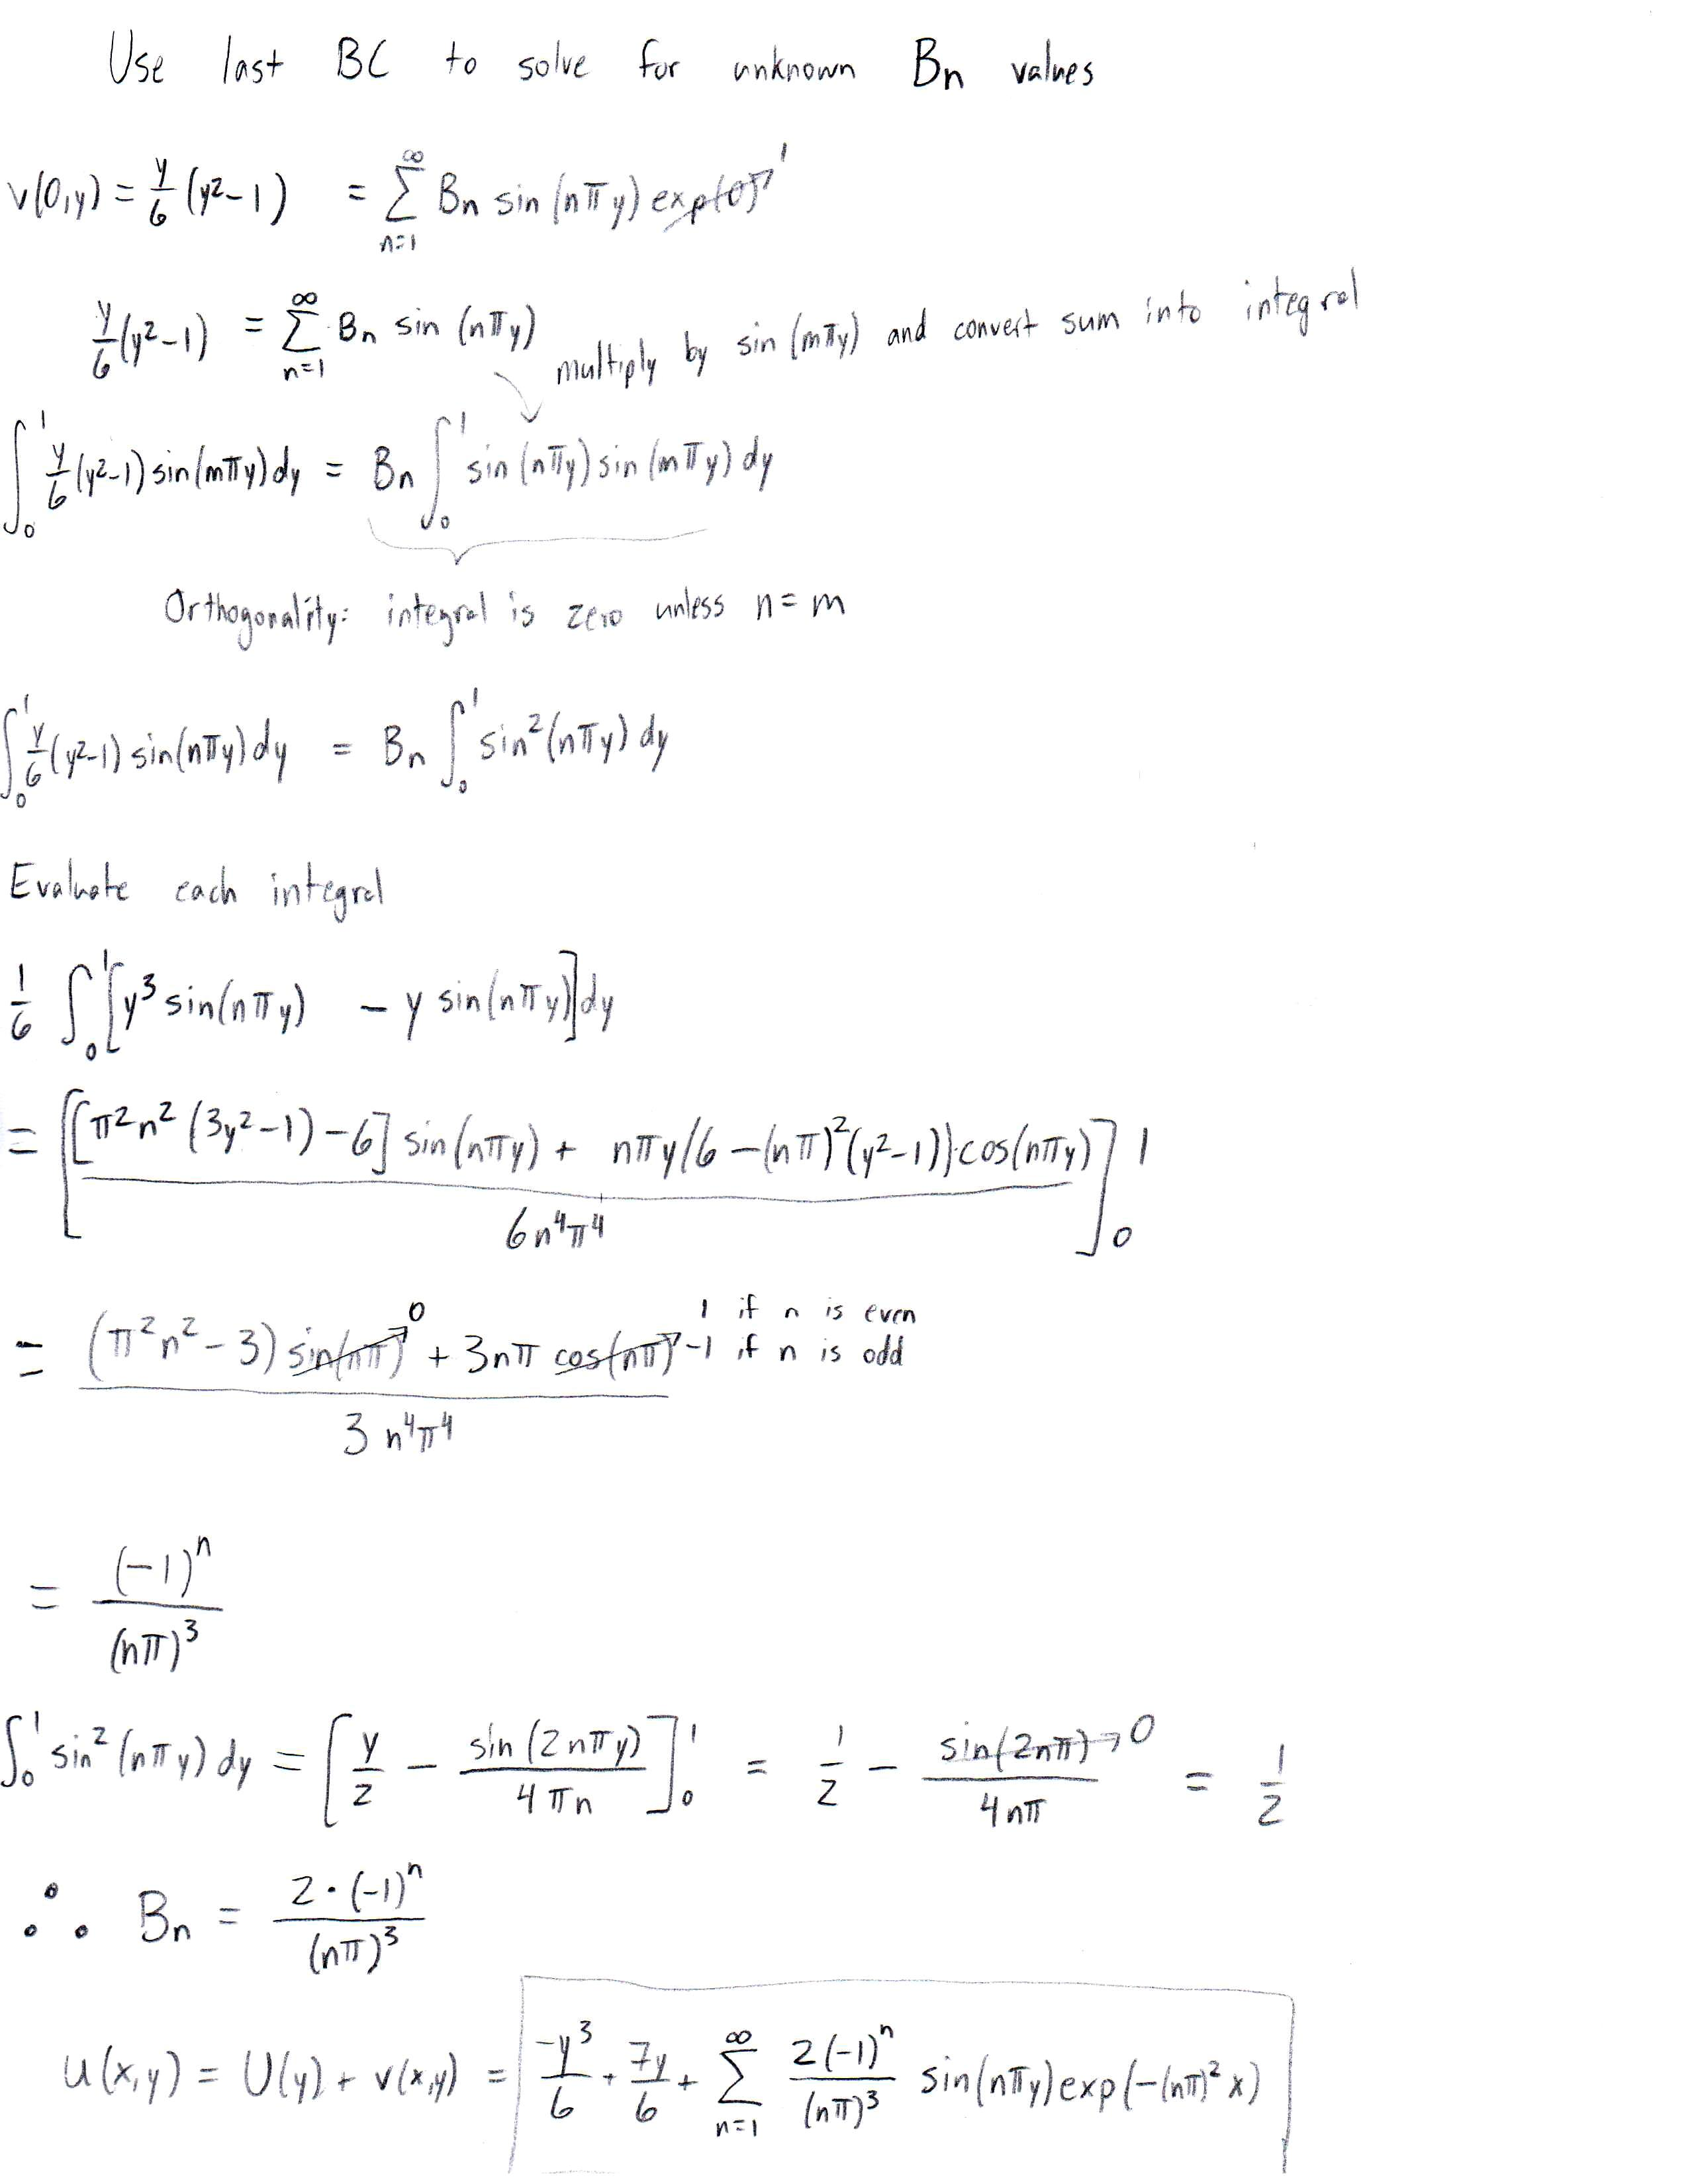
\includegraphics[width=16cm]{app2_p3.jpg}
	\end{center}
\end{figure}
\pagebreak


\section*{Appendix 3: Derivation of Crank-Nicolson Algorithm with 4th-Order accuracy in y}
\begin{figure}[H]
	\begin{center}
		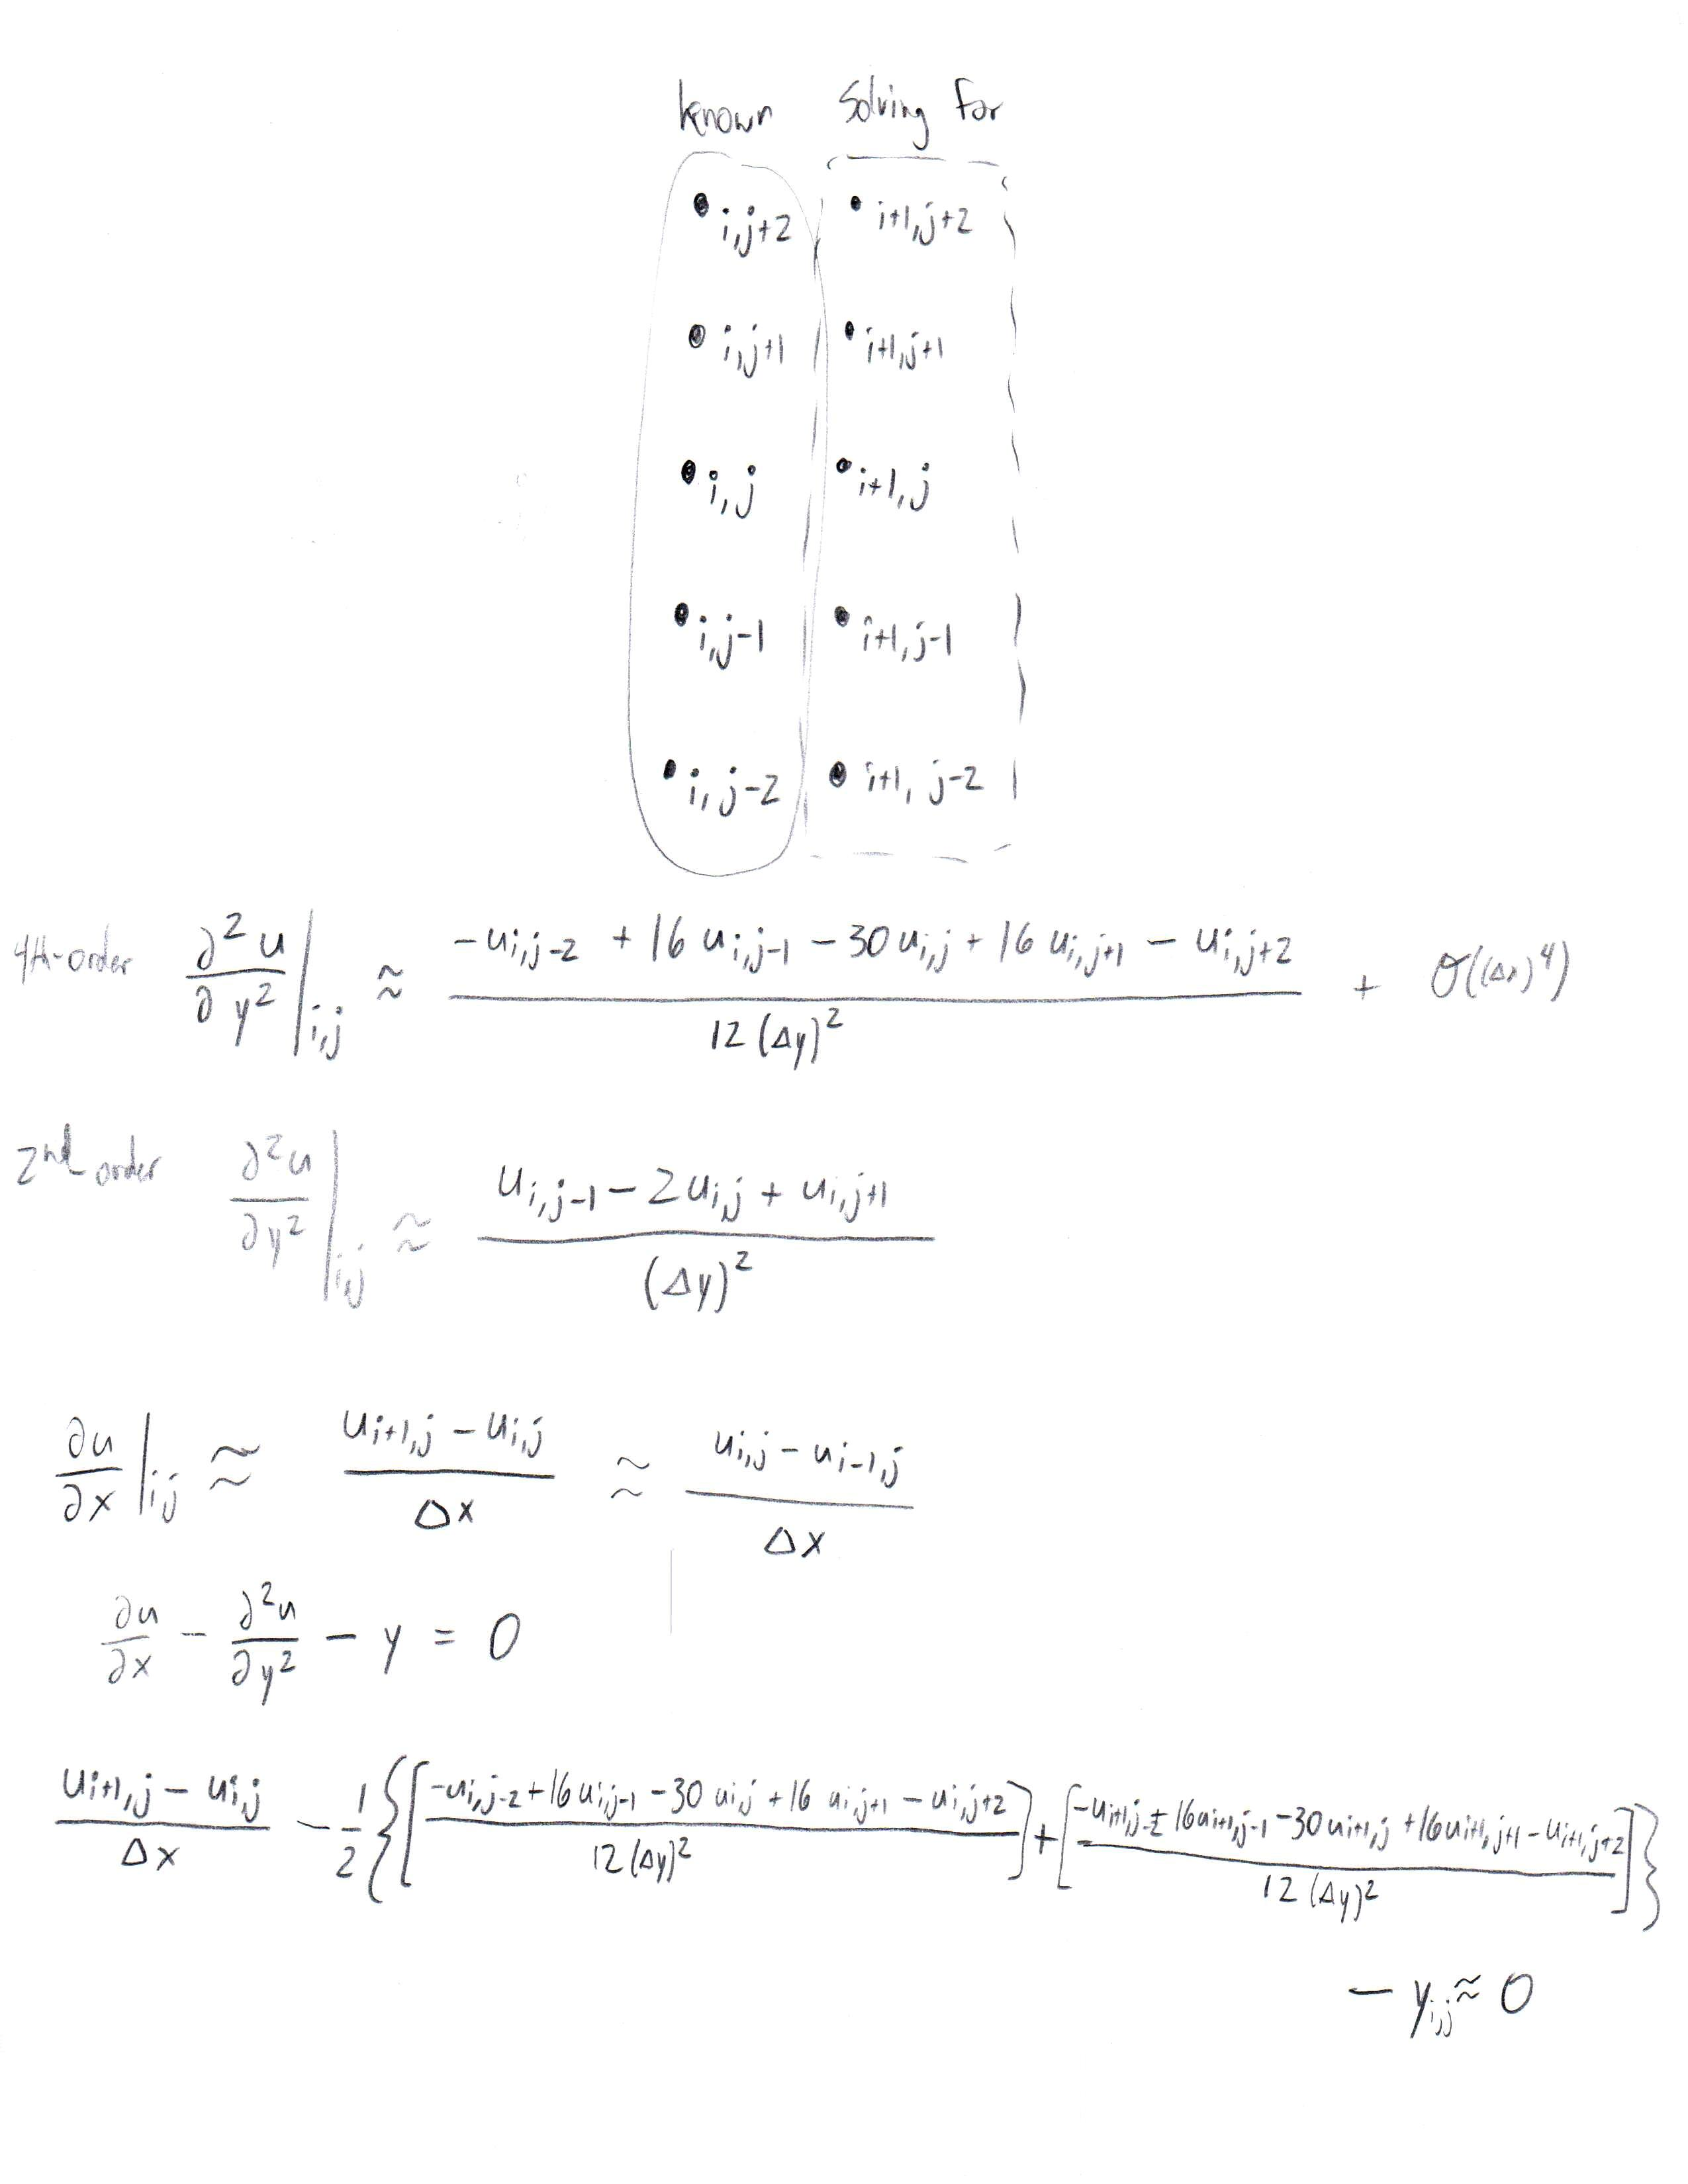
\includegraphics[width=16cm]{app3_p1.jpg}
	\end{center}
\end{figure}
\pagebreak
\begin{figure}[H]
	\begin{center}
		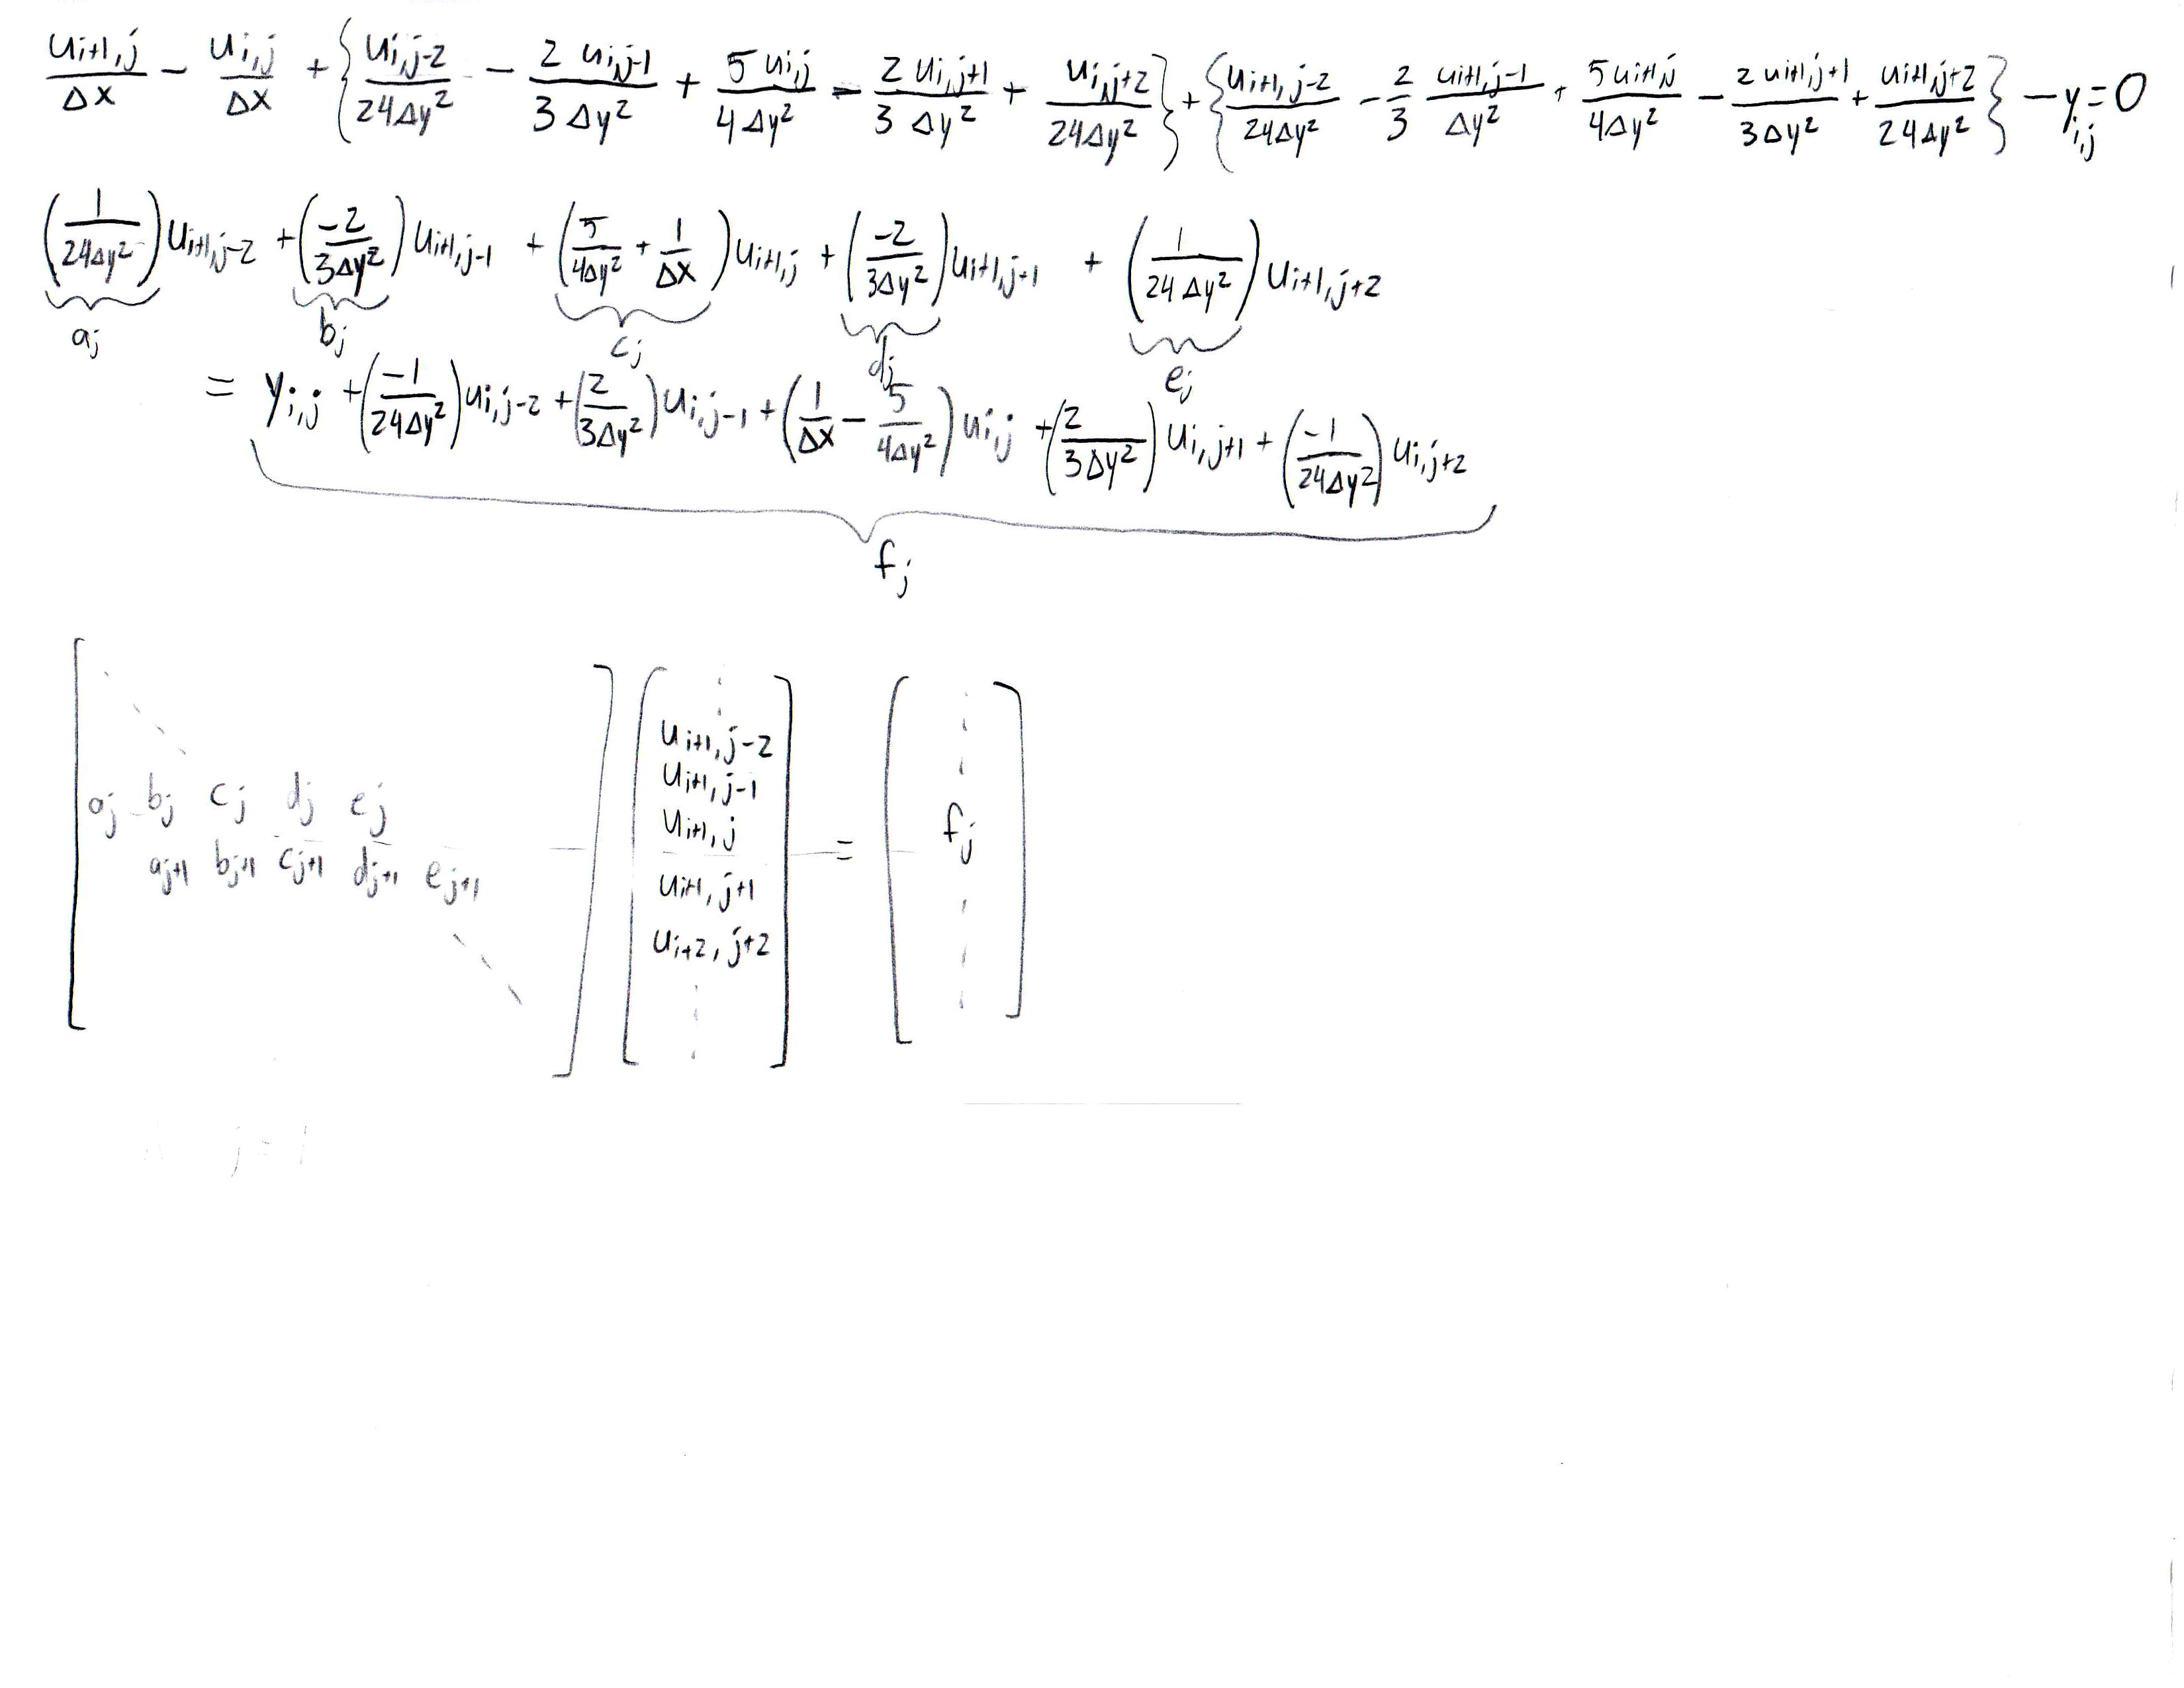
\includegraphics[width=16cm]{app3_p2.jpg}
	\end{center}
\end{figure}
\pagebreak
\begin{figure}[H]
	\begin{center}
		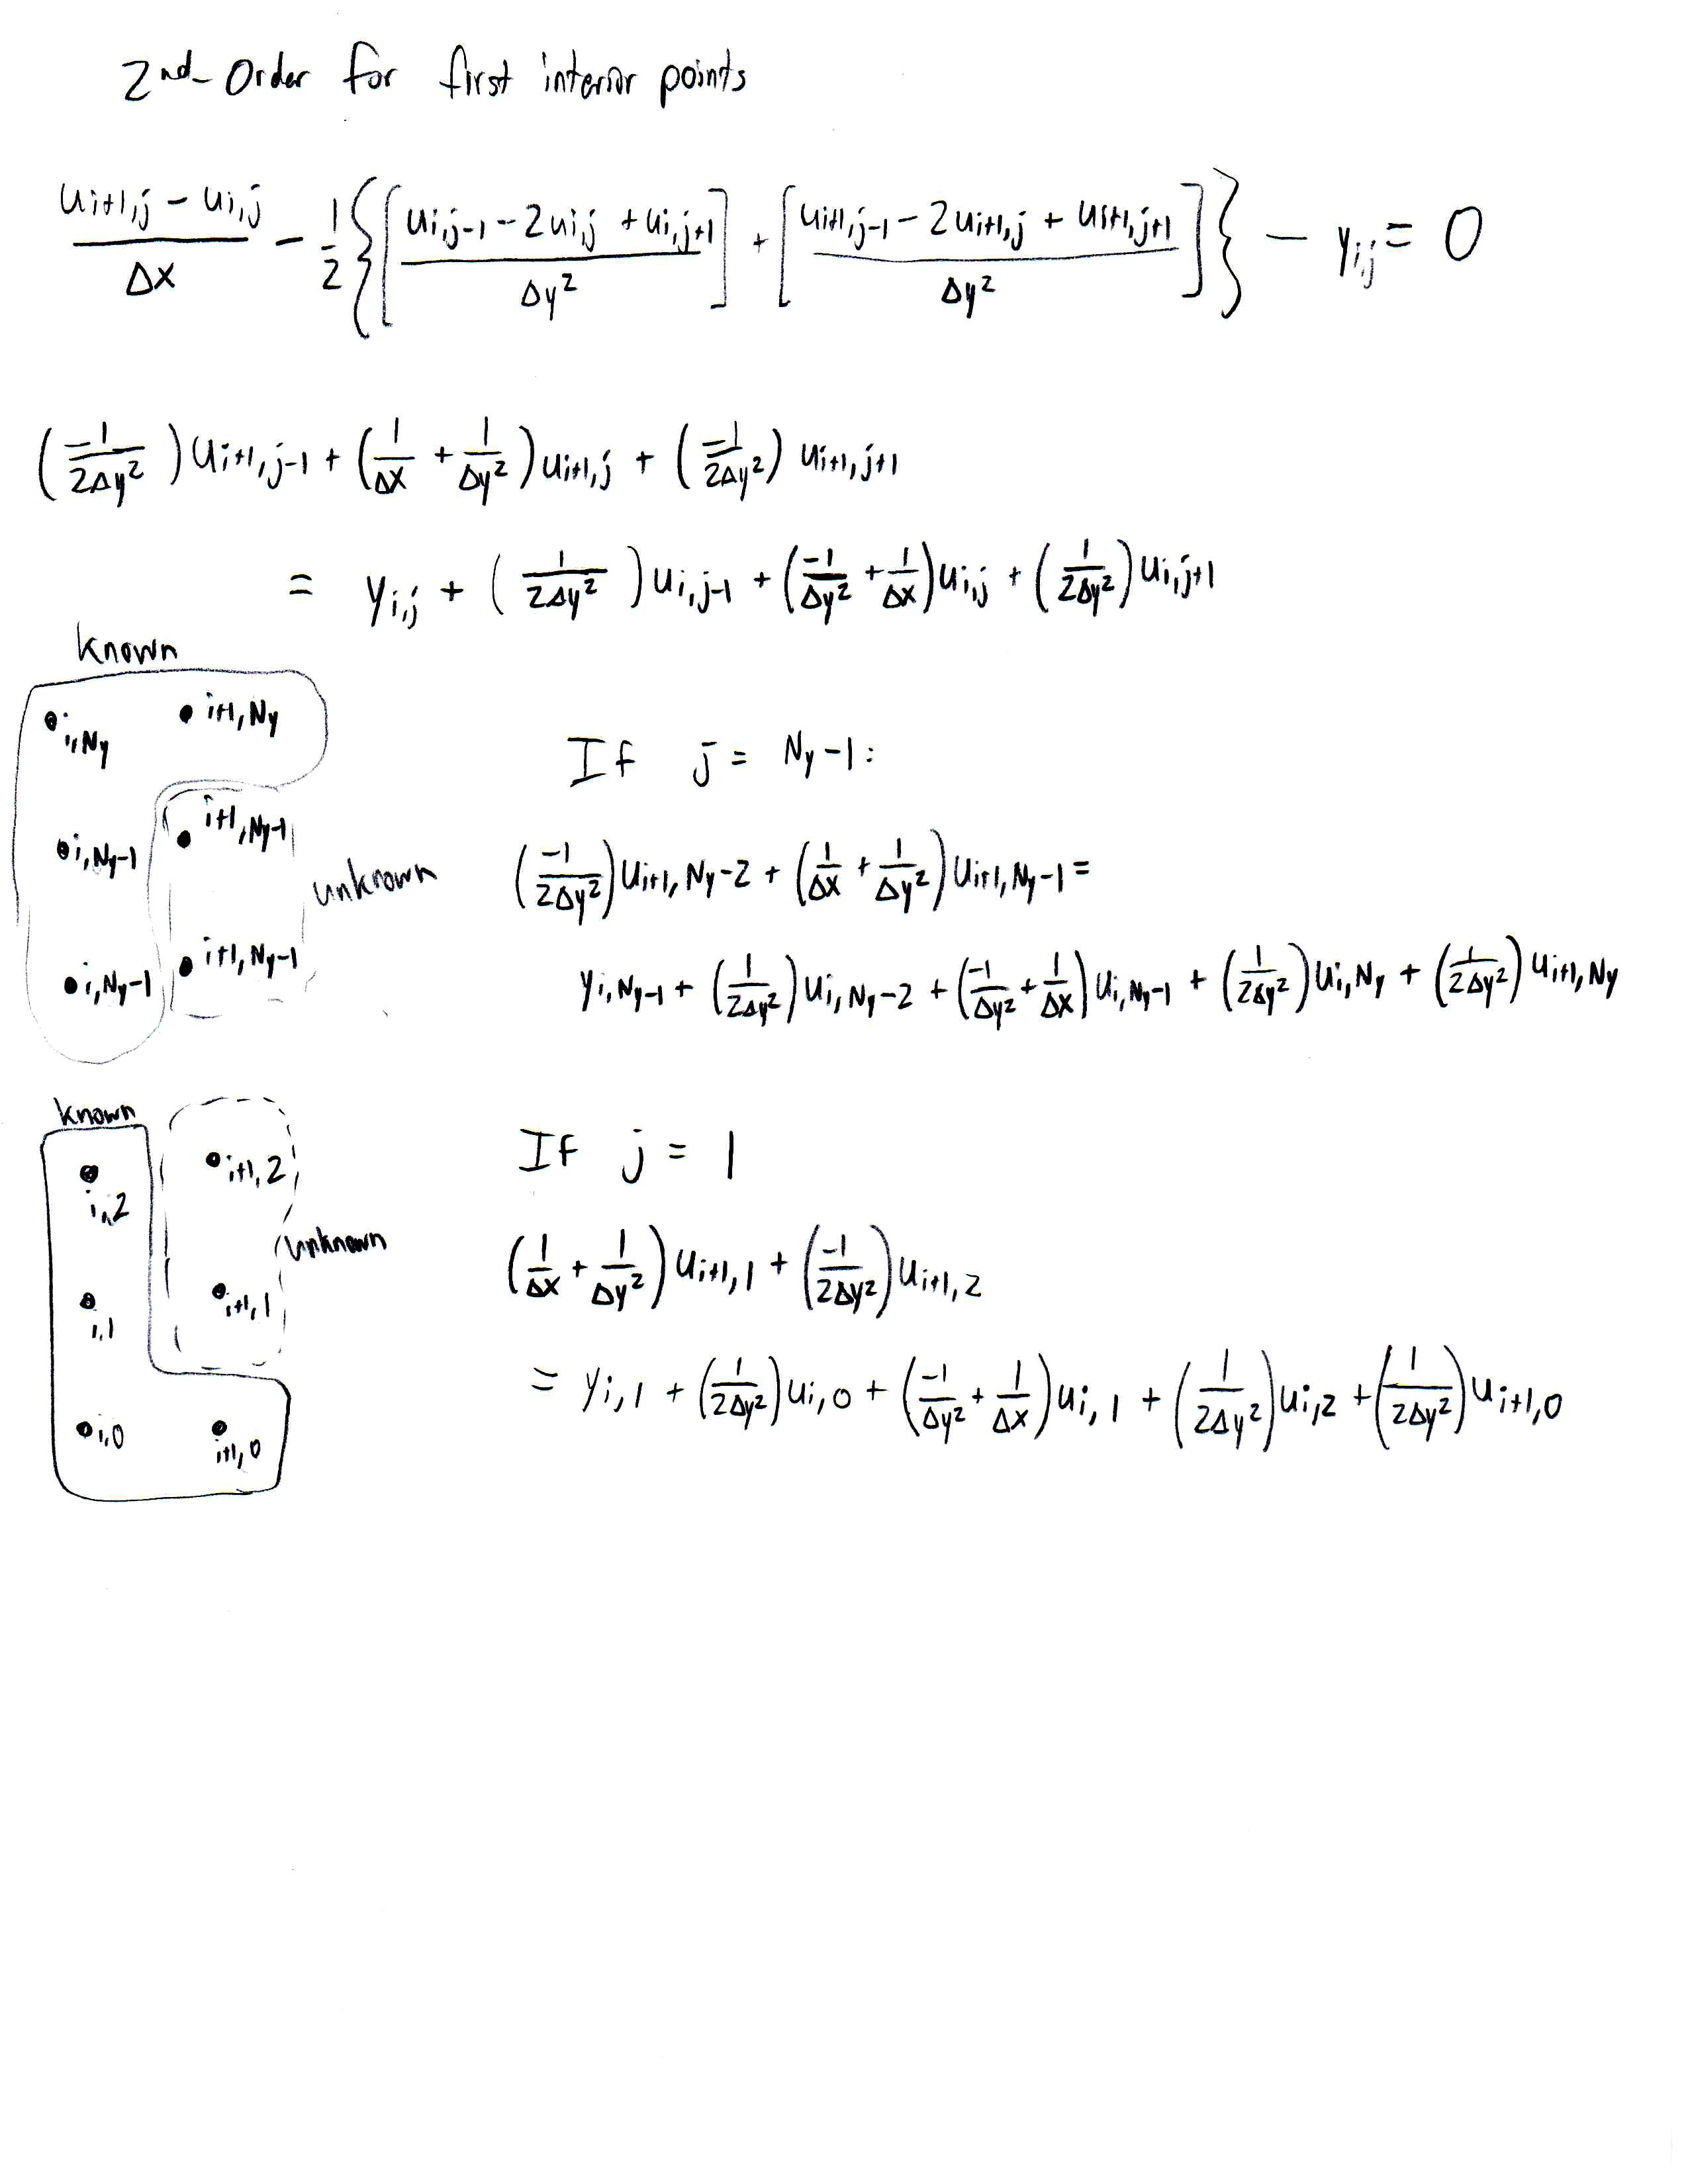
\includegraphics[width=16cm]{app3_p3.jpg}
	\end{center}
\end{figure}

\end{document}

